\documentclass{article}
\usepackage[margin=.75in]{geometry}
\usepackage{setspace}
\linespread{1.5}
\author{Liam M. Sharp}
\title{Proposal for PhD Candidacy\\ Organization and elasticity of membranes containing pentameric-ligand gated ion channels}
\usepackage{graphicx}
\usepackage{mathtools}
\usepackage{color}
\usepackage{amssymb}
\graphicspath{{./Images/}}
\newcommand{\grace}[1]{\textcolor{blue}{#1}}

\usepackage[
   % backend=biber, 
    natbib=true,
    style=numeric-comp,
    sorting=none
]{biblatex}
\addbibresource{./proposal.bib}

\begin{document}
\maketitle
\newpage
\tableofcontents
\newpage
\section{Aims}
Nicotinic acetylcholine receptors (nAChRs) are pentameric ligand gated ion channels (pLGICs) found through out the central and peripheral nervous system. Function of these neurotransmitter receptors is very sensitive to composition of the surrounding lipid membrane. However, the mechanisms of interaction between nAChR and its lipid environment are poorly understood. Research has shown a requirement for cholesterol in reconstitution mixtures of nAChR and other neuronal pLGICs, but other potentially essential lipids abundant in native membranes (particularly n−3 polyunsaturated fatty acids or PUFAs) have not been investigated. For my PhD research I propose the following:

\begin{enumerate}
  \item \textbf{Aim 1: Coarse-grained simulations of multiple subtypes of mammalian pLGICs in quasiphysiological membranes}  We observe nAChR partitioning into  n-3 polyunsaturated fatty acid (PUFA)  rich domains with the n-3 PUFA DHA-PE as nAChR's primary boundary lipid. The concentration of n-3 lipids is much lower in membranes, such as Xenopus oocytes,  commonly used in electrophysiology experiments, than in native membranes. I hypothesize adding small concentrations of n-3 is likely to restore the native boundary lipids. I will model various n-3 supplemented quasi-physiological membranes (such as oocytes) to predict those likely to provide a native local environment within the non-native membrane.%, for later testing by an experimental collaborator (Dr. John Baenziger of University of Ottawa). %We observe nAChR partitioning into n-3 (DHA) rich domains with DHA-PE as nAChR’s primary boundary lipid. Xenopus oocytes lipid composition are considerably different from neuronal membranes, but due to the high affinity of DHA chains for nAChR , a modest supplementation scheme is likely to restore the native boundary lipids. We will model various supplementation schemes to predict those likely to provide a native local environment within an oocyte, for later testing by an experimental collaborator (Dr. John Baenziger of University of Ottawa).

  \item \textbf{Aim 2: Investigation of the relative importance of pLGIC sequence vs shape in determining preferred lipid domain} This can be tested by comparing effects on partitioning profiles upon mutation of lipid facing residues versus adjustments in membrane lipid composition. If the effect of the protein's sequence is measured to be greater than its shape, it is likely that pLGICs will display significant variation in partitioning behavior and annular lipid preferences. If the reverse is observed, it is likely that overall pLGIC shape and relative flexibility of domains drives partitioning, and thus all pLGICs may have similar partitioning behavior.%This can be tested comparing effects on partitioning profiles upon mutation of lipid facing residues versus adjustments in membrane lipid composition. If the former has a stronger effect, it is likely that pLGICs will display significant variation in partitioning behavior and annular lipid preferences, while if the latter has a stronger effect, it is likely that overall pLGIC shape and relative flexibility of domains drives partitioning, with similar preferences across the pLGIC family.

  \item \textbf{Aim 3: Development and release of a user-friendly VMD plugin for measuring elastic parameters of heterogenous membranes} %%This package could be of significant use to both chemists and biophysicists. It would allow computational researchers to easily predict the elasticity moduli of a membrane composed of a general lipid mixture. 
  While multiple individuals have developed scripts to determine the fluctuation spectrum of membranes, there is no universal tool computational chemists and biophysicists can use. I will develop a tool to measure elastic parameters and fluctuation spectra within the convenient scripting environment of the VMD software, which will alleviate the daunting nature of solving for the fluctuation spectrum and related moduli.  This tool will assist us in optimizing lipid selections for modeled neuronal membranes; I can adjust lipid species and lipid concentrations to mimic elastic properties of neuronal membranes. 
\end{enumerate}

\newpage
\section{Introduction}
\label{S:1}
% !TEX root = main.tex

The nicotinic acetylcholine receptor (nAChR) is an excitatory pentameric ligand gated ion channel (pLGIC) commonly found in the neuronal post synaptic membrane and neuromuscular junction (NMJ) in mammals %\cite{Breckenridge_Adult_1973,Cotman_Lipid_1969}, 
as well as the electric organs of the \textit{Torpedo} electric ray. %\cite{Bara89,Quesada_Uncovering_2016} . 
%nAChR is found at especially high concentrations (about $10^4$ $\mu m^{-2}$) within the NMJ membrane \cite{Breckenrldge1972}. 
%The pLGIC super family has been shown to play roles in cognition \cite{Walstab2010}, inflammation \cite{Patel2017,Yocum2017,Cornelison2016}, addiction \cite{Cornelison2016}, chronic pain \cite{Xiong2012} and numerous diseases including: Alzheimer's Disease, spinal muscular atrophy, and neurological autoimmune disease \cite{MartinRuiz_4_1999, Arnold_Reduced_2004,Lennon_Immunization_2003,Papke_The_2012,Picciotto_Neuroprotection_2008}.\grace{this sentence and citations are weird, aren't inflammation and addiction etc diseases?} nAChR plays a major role in excitation of the central and peripheral nervous system and binds agonists such as nicotine, acetylcholine and general anesthetics in multiple sites \cite{Bondarenko_NMR_2013,Jayakar_Identification_2013,LeBard_General_2012,Brannigan_Multiple_2010}.\graceforgrace{fix references here}
nAChRs play a fundamental role in rapid excitation within the central and peripheral nervous system, and neuronal nAChRs are also critical for cognition and memory \cite{Dani2001b, Changeux2015}. Acetylcholine is the orthosteric \nachr~ligand, but numerous other exogenous and endogenous small molecules modulate \nachr s, including nicotine, general anesthetics, the tipped-arrow poison curare,  phospholipids, cholesterol, and cholesterol-derived hormones.\cite{Klaassen2015,Taly2009}  %bind binds agonists such as nicotine, acetylcholine and general anesthetics in multiple sites \cite{Bondarenko_NMR_2013,Jayakar_Identification_2013,LeBard_General_2012,Brannigan_Multiple_2010}.\graceforgrace{fix references here} 
The larger pLGIC super family that includes \nachr s has been shown to play roles in numerous diseases related to inflammation, \cite{Patel2017,Yocum2017,Cornelison2016}, addiction \cite{Cornelison2016}, chronic pain \cite{Xiong2012}, Alzheimer's Disease \cite{Walstab2010,Picciotto_Neuroprotection_2008,MartinRuiz_4_1999}, spinal muscular atrophy \cite{Arnold_Reduced_2004}, schizophrenia \cite{Haydar2010} and neurological autoimmune diseases \cite{Lennon_Immunization_2003}.

nAChRs are highly sensitive to the surrounding lipid environment\cite{Hamouda2006a,Baenziger2017,Padilla-Morales2016,Barrantes2007} for reasons that remain poorly understood. In 1980 it was observed that \nachr s only conduct at native levels if model phospholipid membranes contain 10-20\% cholesterol
\cite{Dalziel1980,Criado1982,Ochoa1983}. Three generations of investigation have followed, with the first generation of studies\cite{Marsh1978,Dalziel1980,Marsh1981,Criado1982,Gonzalez-Ros1982,McNamee1982,Ellena1983,Ochoa1983,Zabrecky1985,Bristow1987,Leibel1987,Middlemas1987,Jones1988a,Jones1988, Fong1986,Fong1987,McNamee1988, Barrantes1989,Sunshine1992,Sunshine1994,Narayanaswami1993,Addona1998,Corbin1998,Barrantes2000} focused on differentiating between the role of bulk, annular, and non-annular cholesterol, a second generation\cite{Baenziger2015,Bruses2001,Marchand2002,Oshikawa2003,Pato2008,Zhu2006,Baenziger2017, Barrantes2007,Barrantes2000,Barrantes2010,Bermudez2010,Perillo2016,Wenz2005,Borroni2016, Unwin2017} probing membrane-mediated effects on organization of multiple \nachr s, and a third generation\cite{Basak2017,Althoff2014,Laverty2017,Zhu2018} applying x-ray crystallography and high-resolution cryo electron microscopy to directly observe lipid binding modes. 

Members of the pLGIC family other than \nachr~are also lipid-sensitive,\cite{Dunn1989,Sooksawate2001,Baenziger2011, Dostalova2014} and lipids other than cholesterol can also modulate function\cite{Bhushan1993,Cheng2007,Corrie2002a,DaCosta2002,Rankin1997,Wenz2005,Hamouda2006a}, but these mechanisms have not been as extensively studied.  The recent publication of several crystal and cryo-EM structures \cite{Basak2017,Althoff2014,Laverty2017,Zhu2018}
has confirmed that specific lipid-pLGIC interactions extend beyond cholesterol and \nachr.  Such interactions are also well-established in other transmembrane proteins, including G-protein coupled receptors (GPCRs) and other ion channels, as reviewed in \cite{Burger2000, Lee2004, Pucadyil2006a, Landreh2016, Smithers2012}. 

Even in the specific case of cholesterol-\nachr~ interactions, results from different approaches have suggested complex behavior and even contradictory interpretations.  Results have indicated that both cholesterol encrichment\cite{Dalziel1980,Criado1982,Ochoa1983} and cholesterol depletion\cite{Santiago2001} cause gain of function, that anionic phospholipids are unnecessary for native function\cite{Dalziel1980,Criado1982,Ochoa1983} or must be\cite{Corrie2002a,DaCosta2002} included in a reconstitution mixture,  that cholesterol increases \nachr~clustering\cite{Pato2008, Zhu2006, Barrantes2007} and directly interacts with \nachr~\cite{Leibel1987,Jones1988}, but \nachr~does not consistently partition into cholesterol-rich domains\cite{Bermdez_Partition_2010}. We suggest here that some of these apparent contradictions may be explained by competition between cholesterol and other lipids found in native membranes, primarily lipids with polyunsaturated fatty acyl chains (PUFAs).   

Interactions of \nachr~ with PUFAs have not been systematically investigated experimentally, but a large amount of circumstantial experimental evidence suggests an important role for PUFAs in \nachr~ function.    Clinically, long-chain $n-3$  (commonly called ``Omega-3'' or $\omega-3$) lipids have a neuroprotective role\cite{Piomelli2007}, and \nachr-associated pathologies can arise for patients with low levels of $n-3$ PUFAs. $\alpha7$ \nachr s are implicated in schizophrenia\cite{Haydar2010}, and dietary supplementation with $n-3$ fatty acids (usually through fish oil) can reduce the likelihood of psychosis, with dramatic effects in some individual cases.\cite{Amminger2010}   

{\it In vitro}, PUFA-rich asolectin\cite{Regost2003,Olsen2003} is one of the most robust additives\cite{Criado1982} for obtaining native \nachr~function. The specific component(s) of asolectin responsible for conferring function have not been identified. 
%The dearth of data is likely due the fact working with polyunsaturated fatty acids (PUFAs) in the laboratory introduces challenges due to lipid peroxidation.  Nonetheless, 
Long chained $n-3$  (previously termed $\omega-3$)  PUFA lipids are abundant in two seemingly disparate \nachr~native membranes: mammalian neuronal membranes\cite{Breckenridge_Adult_1973,Cotman_Lipid_1969} and those of the \textit{Torpedo} electric organ,\cite{Barrantes1989,Quesada2016}. Both such membranes also have an abundance of phosphoethanolamine (PE) headgroups and saturated glycerophospholipids, and a scarcity of monounsaturated acyl chains and sphingomyelin compared to \textit{Xenopus} oocyte membranes \cite{Hill_Isolation_2005} common in functional studies, or even a ``generalized'' mammalian cell membrane \cite{Inglfsson_Lipid_2014}.    % and has been shown to be functionally dependent on cholesterol and anionic lipids when reconstituted into a membrane \cite{Fong_Correlation_1986,Sunshine_Lipid_1992,Hamouda_Assessing_2006,Butler_FTIR_1993,Bhushan_Correlation_1993,Fong_Stabilization_1987,Bednarczyk_Transmembrane_2002,Corrie_Lipid_2002}. The absence of native cholesterol concentrations does not inhibit ligand-nAChR binding, but does prevent gating \cite{Baenziger2015,Carswell_Role_2015,Calimet2013}, impeding ion flux through the pore \cite{Fong_Correlation_1986,Sunshine_Lipid_1992,Hamouda_Assessing_2006,Butler_FTIR_1993,Bhushan_Correlation_1993,Fong_Stabilization_1987,Bednarczyk_Transmembrane_2002,Corrie_Lipid_2002,Cheng_Anionic_2009}. \grace{references} Previous research suggests cholesterol may be bound within the inter- and intra-subunits of the transmembrane domain (TMD) \cite{Brannigan_Embedded_2008}; and cholesterol has been hypothesized and recently found bound within the $\gamma$-Aminobutyric acid receptors (GABAARs) TMD \cite{Hnin_A_2014,Laverty2017}. \grace{add new Hibbs citation} 
%\grace{The first and second generation of studies primarily focused on cholesterol, while the third generation has been focused on any lipids which are resolved in high resolution structures, including cholesterol or phospholipids.  }
% Adding cholesterol to the model membrane increases the ability of the channel to gate, with
%an EC$_{50}$ of 10\% cholesterol and a Hill coefficient of 2 \cite{Rankin1997}.  
%Results suggesting direct interactions between cholesterol and the \nachr, included (1) a pool of cholesterol that cannot be depleted from native Torpedo \nachr-rich membranes,\cite{Leibel1987} (2) quenching of intrinsic nAChR fluorescence by bromocholesterol \cite{Jones1988}  (3)  \nachr-local boundary lipids with rotational correlation times an order of magnitude slower than those in the bulk %with the spin label 14-PCSL, %exchanged with the bilayer at a rate of 6 $\times 10^7$s$^{-1}$  

%demonstrated specific binding of lipids to pLGICs, including Didocosahexaenoyl (DHA) bound Gloeobacter Ligand-gated Ion Channel (GLIC)\cite{Basak2017}, Palmitoyloleoylphosphatidylcholine (POPC) bound Glutamate-gated Chloride Channel (GluCl)\cite{Althoff2014}, and cholesterol-hemisuccinate bound  $\gamma$-aminobutyric acid (A) (GABA(A)) receptor\cite{Laverty2017,Zhu2018}\liam{. In} some cases\cite{Althoff2014, Zhu2018} density deep within the TMD bundle is assigned to phospholipid headgroups\cite{Althoff2014} or cholesterol hemisuccinate\cite{Zhu2018}.   

% and (4) spin labeled lipids indicated the steroid had a higher affinity for \nachr~ than monounsaturated phosphatidylcholine (DOPC) \cite{Abadji1994}.  
%This titration agrees well with the . 
%Action of general anesthetics on the nAChR that were present in native membranes or cholesterol-containing bilayers were absent in the model membranes lacking cholesterol, probably because cholesterol was required to support the necessary conformation change \cite{Raines1994};
 % I've always been curious about the data for this abstract (I didn't find it in a ms).
%a.	Shades of John Baenziger?s uncoupled state
%The action of cholesterol on nAChRs was independent of its ability to flip?flop across the bilayer, but was consistent with a binding site near, but not in, the monounsaturated lipid-protein interface \cite{Addona1998}. 
% Steroids of different stereochemistry supported nAChR activation independent of structural features known to be important for modulation of lipid bilayer properties \cite{Addona2003}.
%A boundary  lipid local to the \nachr, probed with the spin label 14-PCSL, exchanged with the bilayer at a rate of 6 $\times 10^7$s$^{-1}$ and had a rotational correlation time an order of magnitude slower than when in the bilayer.\cite{Abadji1993}.
%\end{enumerate}
%I made a few changes to the above to make them more precise with regard to saturation, please let me know if anything is incorrect. 
%These studies primarily focused on how cholesterol interacted with \nachrz. %Agonist induced rapid fluorescence quenching on the millisecond time scale. Pharmacological criteria were used to establish the specificity of the flux. In a given set of vesicles, the amplitude of flux depended on agonist concentration and a concentration-response curve could be obtained. However, the absolute amplitude of flux could not be compared between preparations presumably because of vesicle morphology issues. 
%Measurable ion flux for reconstituted \gabaar was obtained using vesicles containing asolectin:brain (4:1), but not with asolectin alone.\cite{Dunn1989} No systematic study of the effects of lipid composition was made, even in a followup study;\cite{Dunn1994} it is now established that brain lipids contain primarily $\omega-3$ PUFAs, while asolectin contains $\omega-6$ PUFAs.  
%{Furthermore, most such data was collected and interpreted in an era with little information on \plgic structure or awareness of lateral organization in membranes. }  %In this proposal,  {\bf ``boundary''} lipids refers to lipids bound directly to the \plgic, in either annular or non-annular sites, although the latter may be deep within the protein.  
%Nonetheless, PUFA-rich asolectin\cite{asolectin} has served as the most reliable\cite{which?} reconstitution mixture thus far. 

%%%%%%

%Systematic investigations of the mechanism of \nachr~modulation by lipids have primarily focused on cholesterol, with minimal focus on the effects of polyunsaturation-pLGIC interaction. \liam{There have been a number of studies on PUFA ion channel interaction \cite{Landreh2015,Landreh2016,Caires2017,Borjesson2008,Leaf2002,Xiao2005}, however, these channels are not pLGICs. %The incorporation of asolectin, which is rich in PUFAs, into biological models containing \nachr~in order to restore function \cite{RyanSEDemersCNChewJP1996,DaCosta2005,Criado1984}
%The dearth of data} is likely due the fact working with polyunsaturated fatty acids (PUFAs) in the laboratory introduces challenges due to lipid peroxidation.  Nonetheless, long chained $n-3$  (previously termed $\omega-3$)  PUFA lipids serve as a distinctive common element of two seemingly disparate \nachr~native membranes: mammalian neuronal membranes\cite{Breckenridge_Adult_1973,Cotman_Lipid_1969} and those of the \textit{Torpedo} electric organ,\cite{Barrantes1989,Quesada2016}. Both such membranes also have an abundance of phosphoethanolamine (PE) headgroups and saturated glycerophospholipids, and a scarcity of monounsaturated acyl chains and sphingomyelin compared to \textit{Xenopus} oocyte membranes \cite{Hill_Isolation_2005} common in functional studies, or even a ``generalized'' mammalian cell membrane \cite{Inglfsson_Lipid_2014}. PUFA-rich asolectin\cite{Regost2003,Olsen2003} is one of the most robust additives\cite{Criado1982} for obtaining native \nachr~function, but the specific component has not been identified. Finally, long-chain $n-3$ lipids have a neuroprotective role,\cite{Piomelli2007} and supplementation with $n-3$ lipids can significantly reduce the likelihood of psychosis in schizophrenia-susceptible patients.\cite{Amminger2010}   
%It is now established that brain and \textit{Torpedo} membrane PUFAs primarily have $\omega-3$ chains, while asolectin.  
%Native membranes for \nachr s, including post-synaptic membranes and those of the \textit{Torpedo} electric organ, are enriched in phosphoethanolomine (PE) and  $\omega-3$ polyunsaturated fatty acids (PUFAs)\cite{Breckenridge_Adult_1973,Cotman_Lipid_1969,Bara89,Quesada_Uncovering_2016}, especially . 

 %The \liam{\textit{Torpedo} electric organ's membrane phospholipid composition \cite{Bara89,Quesada_Uncovering_2016} is comparable to the  post-synaptic membranes}. \% are similar in lipid composition to the electric organs of \textit{Torpedo} \cite{Bara89,Quesada_Uncovering_2016}.  

Membranes composed of ternary mixtures of saturated lipids, unsaturated lipids, and cholesterol tend to demix into separate domains. Saturated lipids and cholesterol constitute a rigid liquid ordered phase ($\lo$) in which acyl chains remain relatively straight. \liam{ \cite{Feller_Acyl_2008,Yeagle2016115,Cicuta1981,Bleecker2016}} Unsaturated lipids form a more flexible liquid disordered phase ($\ldo$) in which the chains remain fully melted.  %Domain formation has been studied both experimentally and computationally in model membranes \cite{Lingwood_Lipid_2010,Kaiser_Order_2009,Ma_n_2004,Inglfsson_Lipid_2014,Risselada_The_2008}, showing de-mixing of lipids with saturated fatty acids and unsaturated fatty acids \cite{Levental_Polyunsaturated_2016,Lor2015}. 
%Monounsaturated fatty acids contain a single double bond, while PUFA's contain two or more double bonds through their acyl chain. These double bonds make unsaturated lipids both disordered and highly flexible \cite{Lingwood_Lipid_2010,Pato_Role_2008,Risselada_The_2008,Schley_2007,Rawicz_Effect_2000}. 
%PE (a zwitterionic head group) is one of two major head groups, the other being phosphocholine (PC). nAChR-lipid studies using model membranes with zwitterionic head groups have not included PUFAs, instead favoring saturated and monounsaturated fatty acids. %need proper refs
$\lo$ domains are often visualized as signaling ``platforms'', restricting membrane proteins into a high density ``raft'' that travel around the fluid membrane \liam{\cite{Simons1997,Simons2000}}. 

The first generation of studies into the mechanism underlying cholesterol-modulation of \nachr~ were conducted and interpreted in an era preceding the discovery of lipid-induced domain formation in membranes. %Domain formation is as sensitive to phospholipid unsaturation as it is to cholesterol content. 
The second generation explicitly considered potential interactions of \nachr~with lipid domains.  Since direct interaction between \nachr~and cholesterol had been demonstrated in the first generation of studies, a sensible initial hypothesis was that \nachr~persistently partitioned to $\lo$ domains, retaining little contact with unsaturated chains. Conclusive support for this hypothesis has not been found.  %Density and aggregation of \nachr s in cellular membranes is sensitive to cholesterol depletion. 

Barrantes and colleagues\cite{Wenz2005} found that the addition of \nachr~to a domain-forming lipid mixture increased the size of Dipalmitoylphosphatidylcholine/Cholesterol (DPPC/Chol) lipid-ordered domains, which (combined with additional FRET data) was interpreted as indicating \nachr~was embedded in liquid-ordered domains.  Other experiments investigating whether \nachr s partition into lipid microdomains have been largely contradictory. Some\cite{Marchand2002,Stetzkowski-Marden2006,Willmann2006} suggest that \nachr s are associated with microdomains independently of stimulation by other proteins. Other studies\cite{Zhu2006,Campagna2006} found that \nachr s require stimulation by a protein such as agrin to partition into microdomains. Formation and disassembly of the \nachr-rich microdomains is highly sensitive to cholesterol concentration,\cite{Barrantes2007,Bruses2001,Marchand2002,Zhu2006,Pun2002}

These studies suggested a role for cholesterol-induced phase separation, but do not confirm that \nachr~partitions to the cholesterol-rich phase.  To test for an intrinsic \nachr~ domain preference, Barrantes and co-workers checked for enrichment of \nachr s in the detergent resistant membrane (DRM).   \nachr s were not enriched in the DRM of a model, domain-forming mixture (1:1:1  Chol:POPC:sphingomyelin) \cite{Bermdez_Partition_2010} but inducing compositional asymmetry across leaflets did yield \nachr~enrichment in the DRM fraction \cite{Perillo_Transbilayer_2016}.  While more precise and robust experimental methods for determining partitioning preference and specific boundary lipids such as mass spectrometry have been applied for other transmembrane proteins\cite{Gupta2018,Chorev2018}, they have not been applied to complex heteromers like \nachr.  

Fully atomistic molecular dynamics (MD) simulations\cite{Brannigan_Embedded_2008, Cheng2009, Hnin_A_2014, Carswell_Role_2015 } have served as a natural complement to the third-generation structural biology approach, but are limited in their ability to resolve contradictions between first and second generation studies, because lipids are unable to diffuse over simulation time scales.\cite{Ingolfsson2014,Bond2006,Parton2013,Goose2013,Scott2008}.   Efficient lipid diffusion is a requirement for equilibrating domains or detecting protein-induced lipid sorting.    Coarse-grained MD (CG-MD) has been used to great success in a number of simulations for both lipid-protein binding and membrane organization \cite{Bond2006,Scott2008,Parton2013,Goose2013,Iyer2018,Sodt2014}. Here we use this method as a ``computational microscope'' to observe the equilibrium distribution of lipids local to the \nachr~ in a range of binary and ternary lipid mixtures inspired by native membranes.   We observe a remarkable enrichment of polyunsaturated lipids among \nachr~boundary lipids. To our knowledge, these are the first molecular simulations of the \nachr~in non-randomly mixed membranes, and the first study to systematically investigate the likelihood of polyunsaturated lipids as \nachr~boundary lipids. 
\section{Preliminary Data}
Through coarse grained (CG) molecular dynamics simulations, we have analyzed nAChR-lipid interactions within quasi-native membranes using the structure of the nAChR from the electric organ of the Torpedo electric ray derived by Nigel Unwin using cryo-EM in 2005 \cite{Unwin_Refined_2005}. The coarse grained model allows for significantly larger systems to be constructed than using atomistic models. Running simulations over $\mu$s allows CG lipids to diffuse enough for observation of domain formation or protein-induced lipid sorting.

We use the PUFAs Docosahexaenoic acid (22:6 $n-3$) (DHA) and Linoleic acid (18:2 $n-6$) (LA). Nearly all the $n-3$ PUFAs in both synaptic and \textit{Torpedo}'s electric organ have been determined to be DHA \cite{Breckenridge_Adult_1973,Cotman_Lipid_1969,Bara89,Quesada_Uncovering_2016}. LA was a useful test fatty acid; Risselada et al \cite{Risselada_The_2008} showed it a usable PUFA for domain formation using Martini \cite{martini}.

Our simulations show embedded nAChR consistently partitions into the  $l_{do}$ phase. This research explores nAChR's partitioning behavior, boundary lipid affinity, and deep non-annular lipid-protein interactions termed embedding within domain forming membranes. It is our understanding this is the first study applying coarse grained molecular dynamics to nAChR.

\subsection{Methods}
\label{S:2}
% !TEX root = main.tex
\subsection{System Composition}

All simulations reported here used the coarse-grained MARTINI 2.2\cite{martini} topology and forcefield.%, which was necessary for allowing sufficient lipid diffusion to equilibrate mixed membranes.  
~nAChR coordinates were based on a cryo-EM structure of the $\alpha{\beta}\gamma\delta$ muscle-type receptor in native torpedo membrane (PDB 2BG9\cite{Unwin_Refined_2005}). This is a medium resolution structure (4\AA) and was further coarse-grained using the martinize.py script; medium resolution is sufficient for use in coarse-grained simulation, and the native lipid environment of the proteins used to construct 2BG9 is critical for the present study. The secondary, tertiary and quaternary structure in 2BG9 was preserved via soft backbone restraints during simulation as described below, so any inaccuracies in local residue-residue interactions would not cause instability in the global conformation.  

Coarse-grained membranes were built using the Martini script insane.py, which was also used to embed the coarse-grained \nachr~within the membrane. The insane.py script randomly places lipids throughout the inter- and extra-cellular leaflets, and each simulation presented in this manuscript was built separately.  Binary mixed membranes were composed of one saturated lipid species (Dipalmitoylphosphatidylcholine-DPPC or Dipalmitoylphosphatidylethanolamine-DPPE) and cholesterol (CHOL), while ternary mixed membranes also included either two $n-6$ PUFA acyl chains : Dilinoleoylphosphatidylcholine (DLiPC) or Dilinoleoylphosphatidylethanolamine (DLiPE) or two $n-3$ PUFA acyl chains : Didocosahexaenoylphosphatidylethanolamine (DHA-PE) or Didocosahexaenoylphosphatidylcholine (DHA-PC). DHA-PC is not distributed with the MARTINI lipidome, but was constructed in-house using MARTINI DHA tails and PC headgroups). Multiple box sizes were used depending on the goal;  ``small'' boxes were between $22x22x20$ nm$^3$ and $25x25x25$ nm$^3$, with about {$\sim$ 1400} total lipids and {$\sim$ 80000} total beads, and were used primarily to investigate composition trends, ``large'' boxes were about $45x45x40$ nm$^3$ with about {$\sim$ 8,300} total lipids and {$\sim$ 820,000} total beads, and were used primarily to investigate subunit specificity and long-range sorting, and ``very large'' boxes were $\sim$ 75x75x40~nm$^3$ with about {$\sim$ 19,000} total lipids and {$\sim$ 1.8 million} total beads, and were used to verify that partitioning in the $\ldo$ phase did not reflect finite size effects.  

%The saturated lipids used are Dipalmitoylphosphatidylcholine (DPPC), Dipalmitoylphosphatidylethanolamine(DPPE). The PUFAs used were Didocosahexaenoylphosphatidylethanolamine (DHA-PE), Didocosahexaenoylphosphatidylcholine (DHA-PC), Dilinoleoylphosphatidylcholine (DLiPC), and Dilinoleoylphosphatidylethanolamine (DLiPE). Cholesterol (Chol) was the only sterol used. 
%The lipids used are Dipalmitoylphosphatidylcholine (DPPC), Dipalmitoylphosphatidylethanolamine(DPPE), Didocosahexaenoylphosphatidylethanolamine (DHA-PE), Didocosahexaenoylphosphatidylcholine (DHA-PC), Dilinoleoylphosphatidylcholine (DLiPC), Dilinoleoylphosphatidylethanolamine (DLiPE) and cholesterol (Chol).

\subsection{Simulations}


Molecular dynamics simulations were carried out using GROMACS\cite{grom}; small boxes used GROMACS 5.0.6 and large boxes used  GROMACS 5.1.2 or 5.1.4. All systems were run using van der Waals (vdW) and Electrostatics in shifted form with a dielectric constant of $\epsilon_r$=15. vdW cutoff lengths were between 0.9 and 1.2 nm, with electrostatic cutoff length at 1.2 nm.

Energy minimization was performed over 10000 to 21000 steps.  Molecular dynamics were run using a time step of 25~fs, as recommended by MARTINI, for 2 $\mu$s for {small membranes,and 10 $\mu$s for large and very large membranes}. Simulations were conducted in the isothermal-isobaric (NPT) ensemble, by using a Berendsen thermostat set to 323 K with temperature coupling constant set to  1 ps, as well as isotropic pressure coupling with compressibility set to $3\times 10^{-5}$ bar$^{-1}$ and a pressure coupling constant set to 3.0 ps. %All systems were run using van der Waals (vdW) and Electrostatics in shifted form with a dielectric constant of $\epsilon_r=15$. vdW cutoff lengths were between 0.9 and 1.2 nm, with electrostatic cutoff length at 1.2 nm.

%However most energy minimizations finished within $\sim$ 1700 to 3000 steps. Molecular dynamics were run using a time step 0.025 $ps$ for 2 $\mu$s. Simulations used  NPT ensembles. We used Berendsen thermostat with an isotropic pressure couple. The reference temperature was set to 323 Kelvin with temperature coupling constant set to  1 $ps$. The system's compressibility is set to $3e^{-5}$ $bar^{-1}$ and a pressure coupling constant of 3.0 $ps$. 
%\liam{In the case of systems at $45x45x40$ $nm^3$, Martini 2.2 and Gromacs 5.1.2 and 5.1.4 were used. Parameters remain the same, however energy minimization was carried out to $\sim$ 21000 steps, and 12.5 $ns$ of NPT equilibration were performed before $\sim 4.5-5 \mu s$ simulation was performed.}

Secondary structures restraints consistent with MARTINI recommendations were constructed by the martinize.py \cite{martini} script {and} imposed by Gromacs\cite{grom}. Protein conformation was maintained in small systems via harmonic restraint (with a spring constant of 1000 kJ$\cdot$ mol$^{-1}$) on the position of backbone beads. \nachr~conformation in large systems was preserved via harmonic bonds between backbone beads separated by less than 0.5 nm. Based on Martini's \cite{martini} ElNeDyn algorithm \cite{Periole_Combining_2009} with a harmonic constant of 900 kJ$\cdot$ mol$^{-1}$.  These restraints limited the root-mean-squared-displacement (RMSD) of the backbone to less than 2.5 \r{A} throughout the simulation.  

The minimum equilibration time depended on the system size. Small systems typically began domain formation by 500 ns, with domains fully formed by 1000 ns. Large systems and very large simulations required about 5$\mu$s of equilibration for stabilization of $M_{DHA,DHA}$.

\subsection{Analysis}

Extent of domain formation within the membrane was tracked by 
    \begin{equation}
    \begin{aligned}
      M_{A, B} = \frac{\langle n_{A,B} \rangle} {6x_{B}} -1 
    \end{aligned}
    \label{eq:M}
  \end{equation}
 where $n_{A,B}$ is the number of type B molecules among the 6 nearest neighbors for a given type A molecule, and the average is over time and all molecules of type $A$. For a random mixture, $\langle n_{A,B} \rangle = 6x_{B}$, where $x_{B}$ is the fraction of overall bulk lipids that are of type B. ${M_{A,B}~0}$ indicates random mixing while ${M_{A,B}>0}$  and ${M_{A,B}<0}$ indicate demixing and excessive mixing respectively.  

%	$M_{a,b}$ compares measured and expected mixing, where $a$ and $b$ represent a reference and a local lipid species respectively, equation \ref{eq:M}. 
%    \begin{equation}
%    \begin{aligned}
%      M_{a,b} = \frac{\langle \eta_{a,b} \rangle} {\langle \eta_{a,b} \rangle_{rand}} - 1
%    \end{aligned}
%    \label{eq:M}
%  \end{equation}
%  We define $\eta_{a,b}$ as the percentage of lipid species $b$ in contact with lipid species $a$. $M_{a,b}$ is subtracted by one to include all points.

Extent of receptor partitioning within the $\lo$ or $\ldo$ domain was tracked by counting the number $\bsat$ of saturated boundary lipids and comparing with the expectation for a random mixture, via the order parameter $\qsat$:
  \begin{equation}
    \begin{aligned}
      \qsat\equiv \frac{1}{\xsat}\left\langle\frac{  \bsat }{\nbound }\right\rangle-1,\\
    \end{aligned}
    \label{eq:Q}
  \end{equation}
  where $\nbound$ is the total number of lipids in the boundary region and $\xsat$ is the fraction of overall bulk lipids that are saturated phospholipids. $\qsat <0$ indicates depletion of saturated lipids among boundary lipids, as expected for partitioning into an $\ldo$ phase, while $\qsat>0$ indicates enrichment and likely partitioning into an $\lo$ phase. Each frame, $\nbound$ and $\bsat$ were calculated by counting the number of total and saturated lipids, respectively, for which the phosphate bead fell within a distance of 10~\AA~ to 35~\AA~ from the M2 helices, projected onto the membrane plane. 
  
  Two-dimensional density distribution of the beads within a given lipid species $B$ around the protein was calculated on a polar grid: %$\rho_a$ (\r{A}$^{-2}$) is the density of lipid $a$ within a given bin equations \ref{eq:R}.
  \begin{equation}
    \begin{aligned}
      \rho_{B}(r_i,\theta_j)= \frac{\left\langle n_{B}(r_i,\theta_j) \right\rangle}{r_i \Delta{r}\Delta{\theta}} \\        
    \end{aligned}
    \label{eq:R}
  \end{equation}
  where  $r_i = i \Delta{r}$ is the projected distance of the bin center from the protein center, $\theta_j = j \Delta{\theta}$ is the polar angle associated with bin j,  $\Delta{r}$= 10\AA~ and  $\Delta{\theta} = \frac{\pi}{15}$ radians are the bin widths in the radial and angular direction respectively, and $\left\langle n_{B}(r_i,\theta_j) \right\rangle$ is the time-averaged number of beads of lipid species $B$ found within the bin centered around radius $r_{i}$ and polar angle $\theta_{j}$.  In order to determine enrichment or depletion, the normalized density $ \tilde{\rho}_{B}(r_i,\theta_j)$ is calculated by dividing by the approximate expected density of beads of lipid type B in a random mixture, $x_{B}s_{B}~N_{L}/\langle L^{2}\rangle$, where $s_{B}$ is the number of beads in one lipid of species B, $N_{L}$ is the total number of lipids in the system, and $\langle L^{2}\rangle$ is the average projected box area: 
  \begin{equation}
    \begin{aligned}
  \tilde{\rho}_{B}(r_i,\theta_j)=\frac{ \rho_{B}(r_i,\theta_j)}{x_{B}s_{B}~N_{L}/\langle L^{2}\rangle} \\        
    \end{aligned}
    \label{eq:Rt}
  \end{equation}
  This expression is approximate because it does not correct for the protein footprint or any undulation-induced deviations of the membrane area.  The associated corrections are small compared to the membrane area and would shift the expected density for all species equally, without affecting the comparisons we perform here.   
   %However, as a result of smaller boxes, protein-protein interaction across the periodic boundary resulted in a ''pinwheeling'' effect. 

   %To compensate this, $\rho$ was adjusted by the thickness of the membrane
   %\begin{equation}
   % \begin{aligned}
   %   \tilde{\rho}_{B,i}=\rho_{B,i}\left\langle\frac{1}{\til%de{z}_{i}}\right\rangle \\        
   % \end{aligned}
   % \label{eq:Til}
  %\end{equation}
 %, \liam{$\tilde{z}_{i}$ is the thickness of a membrane per total number of lipids in a given bin}. %In the case of Cartesian bins, $A = \Delta{x} \Delta{y}$ where 
 
 %\liam{Regardless of the pinwheeling effect, 
  
\subsection{Results}
\label{S:3}
% !TEX root = main.tex
\begin{figure*}[h!]
	\center
	\includegraphics[width=\linewidth]{DPPC_Only.pdf}
	\caption{nAChR boundary lipids in binary mixtures of DPPC and CHOL. A: Representative frame from a simulated trajectory of a single nAChR embedded in a small membrane, colored by subunit ($\alpha$:green, $\beta$:purple, $\delta$:gray, $\gamma$:cyan) in a 4:1 DPPC (blue):Chol (red) mixture.  B: Extent of demixing ($M_{DPPC,DPPC}$ defined in Eq. \ref{eq:M}) and depletion of saturated lipids from the boundary ($\qsat$ defined in Eq.\ref{eq:Q}) in small binary membranes. In this binary system, cholesterol depletion/enrichment is directly related to the saturated lipid depletion/enrichment: $Q_\mathrm{chol}=-x_{\mathrm{sat}} \qsat/\xch$.  Error bars represent standard error for a blocking average over 50 ns. C: Average normalized density (Eq. \ref{eq:Rt}) of cholesterol for the system in A. Plot shown is identical to Figure \ref{fig:sorting} in ``Chol'' row, ``None'' column, but has been cropped and zoomed around the protein center.\grace{Update previous sentence upon inclusion of new figure}}
	\label{fig:binary}
\end{figure*} 
\subsection {Spontaneous association with cholesterol in binary membranes} \label{binary}

%We previously proposed that cholesterol could be embedded within intersubunit and intrasubunit sites of \nachr\cite{Brannigan_Embedded_2008} or intersubunit sites of the GABA(A) receptor\cite{Brannigan_Embedded_2008}.  It was recently found in \cite{Laverty2017}, to embed within the inter- and intra-subunits of nAChR and other pLGICs. Docking has been used in previous computational research to determine optimal cholesterol binding domains \cite{Hnin_A_2014,Brannigan_Embedded_2008}, but coarse grained systems have shown to be a novel method to simulate non-annular lipid binding without the need to dock lipids within proteins. \liam{Figure \ref{fig:binary} measures an absence of embedded DPPC but an enrichment of cholesterol embedding throughout the protein.}
Lipid sorting was characterized for \nachr s in binary DPPC:CHOL membranes (Figure \ref{fig:binary}A)  using several metrics. 
Non-random lipid mixing (including domain formation) was quantified using the self-association metric $M_{A,A}$ as defined in Equation \ref{eq:M}. %; this quantity reflects degree of self-association of DHA-containing and LA-containing lipids respectively.  %enrichment of lipid species $B$ among the nearest neighbors of lipid species $A$ , with values close to 0 indicating random mixing, and positive and negative values indicating enrichment or depletion of species $B$ around species $A$, respectively. $M_{A,B}>> 0$ indicates substantial demixing and domain formation.  
As expected, in simulated binary membranes containing only DPPC and 0-40\% cholesterol, minimal demixing was observed, with values of $M_{DPPC,DPPC}$ (Fig \ref{fig:binary}B) rising slightly for higher cholesterol concentrations but remaining persistently below 0.05.  %Similar values were observed for $M_{CHOL,CHOL}$.

Depletion of saturated lipids among \nachr~boundary lipids (relative to those expected for a random mixture) was quantified using the metric $\qsat$ defined in equation \ref{eq:Q}. Negative and positive values of $\qsat$ reflect depletion or enrichment of saturated lipids in the \nachr~boundary, respectively. In binary systems containing cholesterol and saturated lipids, depletion of saturated lipids corresponds directly to enrichment of cholesterol: $Q_{chol} = -\qsat x_{sat}/\xch$. %, respectively, while values of $\qsat$ approaching 1 or -1 indicates partitioning within a well-defined $\lo$ or $\ldo$ phase, respectively.

In binary DPPC:CHOL mixtures, $\qsat$ was very slightly negative for $\xch < 20\%$, but decreased steadily for higher concentrations. This trend indicates some depletion of DPPC (and enrichment of cholesterol) among \nachr~ boundary lipids (Figure \ref{fig:binary}B).  Typically, between 10 and 20\% cholesterol has been required in reconstitution mixtures to restore native function  \cite{Fong_Correlation_1986,Dalziel1980,Criado1982}  and a phase transition at about 20\% cholesterol in binary DPPC:CHOL model membranes is indicated by differential scanning calorimetry.\cite{Marsh2010} 

Spontaneous binding of cholesterol to non-annular or ``embedded'' sites, similar to what we previously proposed\cite{Brannigan_Embedded_2008}, was observed in these CG-simulations, and penetration of the TMD bundle by DPPC acyl chains was also observed at lower cholesterol concentrations (Fig \ref{fig:binary}A).  Distribution of density for embedded lipids is further discussed in Section 3.4.  %deep binding of lipids was much more common in the subunit interfaces, particularly $\alpha/\beta$ and $\delta/\alpha$, than in the subunit center (Figure \ref{fig:sorting})\liam{. A}lthough DPPC partitioned extensively to the relatively large cavity in the center of the $\beta$ subunit.  

Annular cholesterol (enrichment of cholesterol at the protein-lipid interface), is visible for the binary systems via a ring of high (red) cholesterol density just around the protein in Figure \ref{fig:binary}C. Enrichment of cholesterol near the protein is highly localized with a ring that is less than 5\AA~wide. This is in general agreement with evidence for annular cholesterol in randomly-mixed binary membranes. \cite{Barrantes2010}

%at low concentrations of cholesterol, \liam{it is} almost entirely within ``embedded'' or non-annular \liam{region of the protein} (Figure \ref{fig:binary}C) as predicted in \cite{Brannigan_Embedded_2008}.
%Intriguingly, all simulations consistently yielded four general regions of differential embedded cholesterol density : a high density region ($\alpha_{\gamma}/\gamma$ interface and center of the $\alpha$ subunit), a low/background density region ($\beta/\alpha_{\gamma}$ interface and center of $\beta$ subunit) on the opposite face of the TMD, and two regions of intermediate density that separated them.  In the absence of nAChR, DPPC/CHOL lipid bilayers are randomly mixed, so this result indicates an intrinsic cholesterol amphipathy.  

%At higher concentrations of cholesterol, cholesterol was also enriched in ``annular'' sites, particularly at the high affinity and low affinity face of the TMD.  This enrichment actually extended many lipidation shells off the high affinity face, indicating nAChR was not just sorting lipids, but even inducing organization of the membrane. Enrichment far from the TMD is expected to be particularly sensitive to finite size effects, although there is no clear reason for why these effects would consistently have a dependence on protein orientation.  
% , and two intermediate density regions (1: $\gamma-/\alpha+$ face and subunit center of both subunits and 2: ) and $\delta-/\alpha+$ faces, and nearly background density on the $\alpha-/\beta+$ face.  As a result, the protein overall 


\subsection {Domains formed in PUFA-containing ternary membranes are not affected by introduction of an \nachr } \label{Demix}
	\begin{figure}[h!]
		\center
		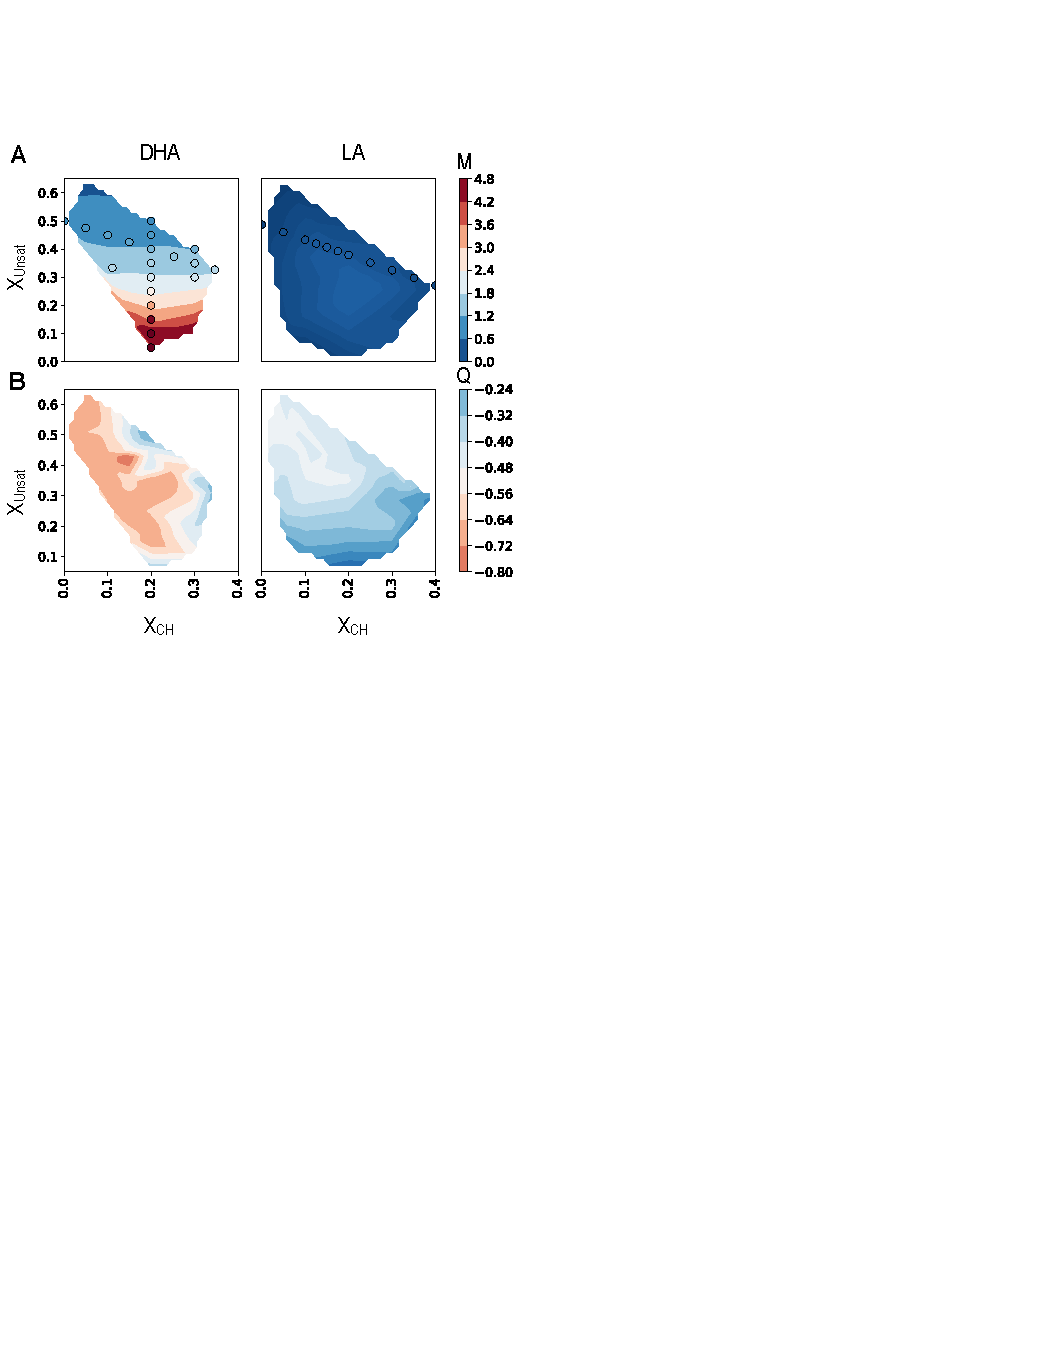
\includegraphics[width=1\linewidth]{Fig2.pdf}
		\caption{Quantitative analysis of bulk membrane mixing and nAChR boundary lipid composition across small membranes containing DPPC, Cholesterol, and either dDHA-PE or dLiPC. Shaded contours were constructed based on 40 individual simulations with DHA and 30 with LA. A: $M_{PUFA, PUFA}$, defined in eq \ref{eq:M}.  Circles represent mixing of systems with the same lipid composition but no \nachr. B: $\qsat$, defined in Eq \ref{eq:Q}.   }
		\label{fig:fig2}
	\end{figure} 
	
	In order to test whether \nachr~affected domain formation in domain-forming membranes, we characterized $M_{{PUFA,PUFA}}$ for systems containing DPPC, Cholesterol, and PE or PC with either n-3 (DHA) or n-6 (LA) acyl chains.   Addition of phospholipids with unsaturated acyl chains to systems containing a saturated lipid and cholesterol is well-established to induce domain formation, and polyunsaturated phospholipids make these domains more well-defined\cite{Levental_Polyunsaturated_2016}. As expected, we observed that addition of PUFAs to DPPC/CHOL bilayers did induce domain formation over a range of compositions, and values for $M_{{PUFA,PUFA}}$ are shown as filled symbols in Figure \ref{fig:fig2} A. 
	
	Introducing a single nAChR to these same systems did not significantly affect domain formation. $M_{DHA,DHA}$ was determined for an isolated \nachr~in ternary mixed membranes with over 40 different combinations of DHA, DPPC, and Cholesterol (Figure \ref{fig:fig2}A, shaded contours). Its effect on membrane organization is represented by the difference in color of the circular symbol and the shaded contour at the same composition.  Introducing a single nAChR into the DHA-containing systems does slightly reduce the amount of DHA required to obtain a given value of $M_{DHA,DHA}$. %, %the difference increased at high DHA concentrations (i.e. $\sim \geq30\%$) and
	%which
	{ This subtle trend} may reflect increased likelihood of DHA-DHA interactions due to nucleation of DHA-containing lipids around the protein (Figure \ref{fig:fig1}). 

	Across ternary mixtures with two long $n-3$ PUFA chains (DHA) and a PE headgroup, maximum values of $M_{DHA,DHA}$ approached 5 (Figure \ref{fig:fig2}A), and were significantly reduced (to less than 0.5) when DHA chains were replaced with linoleic acid (LA) chains. This result is consistent with a previously-observed significant increase in miscibility temperature upon supplementation of plasma membranes with $n-3$ lipids.  \cite{Levental_Polyunsaturated_2016} 
	
	Substantial lipid demixing in DHA-containing mixtures was observed even at low cholesterol concentrations. Over the range we tested, $M_{DHA,DHA}$ was not sensitive to cholesterol concentration $\xch$, as shown by the horizontal contours for DHA in Figure \ref{fig:fig2}A.   
	%	
%	As shown in Figure \ref{fig:fig2}\textbf{a},  $M_{DHA,DHA}$ actually increases as the molar fraction of DHA-PE is reduced from the membrane, implying increased self-association of DHA at reduced concentrations of DHA, with even the lowest concentrations of DHA that we used here seemingly higher than the critical miscibility concentration.  $M_{DHA,DHA}$ is not sensitive to the ratio of cholesterol vs saturated lipid, at least over the compositions simulated.   Relative to systems containing DHA, $M_{LA,LA}$ implies miscibility fo systems containing LA, with small amounts of domain formation sensitive to the CHOL:DPPC ratio; an apparent maximum for $M_{LA,LA}$ occurs near 20\% LA, 20\% Cholesterol, and 60\% DPPC.  
	%This is consistent with previous work, \cite{Inglfsson_Lipid_2014,Risselada_The_2008,Perlmutter_Interleaflet_2011,Veatch_Organization_2002}, indicating domain formation in ternary mixtures to be primarily dependent on differences in acyl chain unsaturation and relatively insensitive to head group.
%The well-defined boundaries between domains that were found in systems containing DHA-PE are also observed in systems containing DHA-PC. Shorter acyl chains and greater saturation did not promote well defined domains as seen using DHA (see Figure \ref{fig:fig1}A). DHA is a relatively long chained n-3 fatty acid making it highly flexible. DHA has been shown to stabilize $\ldo$ domain formation \cite{Levental_Polyunsaturated_2016,Lor2015}.  It may be the case running our simulations for longer time would produce well defined domains for any DLiPC/PE \cite{Risselada_The_2008}.

\subsection{nAChR consistently partitions to the liquid disordered domain} \label{PUFA}
	For more than 100 lipid compositions tested, nAChR always partitioned into a PUFA-rich $\ldo$ phase if such a phase was present. We never observed \nachr~partitioning to an $\lo$ phase. Representative frames from trajectories of domain formation in the presence of \nachr~are shown in Figure \ref{fig:fig1}.  This observation includes all tested concentrations of the ternary mixtures, regardless of whether the zwitterionic headgroup was PC or PE (Figure \ref{fig:SIQ}), or whether DPPC was replaced by dioleoylphosphatidylcholine (DOPC) (di-18:1), Palmitoyloleoylphosphatidylcholine (POPC) (16:0,18:1), or dilauroylphosphatidylcholine (DLPC) (di-14:0), as shown in Figure SI\ref{fig:OL}.   %\liam{This is independent of acyl chain length, but dependent on the level of unsaturation, as seen in .} If PUFAs were included, unsaturated lipids were enriched and saturated lipids depleted from the boundary.}  
	
	% within a randomly mixed ternary membrane, then allowing the membrane to de-mix and nAChR to explore domains, reveals nAChR to partition into the $l_d$ domain if a $l_d$ domain is present. 
		%	Similarly, %\ref{fig:OL}, 
	%partitioning to the disordered domain was qualitatively insensitive to headgroup (PE or PC) for the compositions simulated. 
	%In  heat maps describing the boundary DPPC near nAChR. 
	{These results are quantified for \nachr~embedded in ternary membranes containing DPPC, CHOL, and either DHA-PE or dLiPC\grace{We repeatedly use LA rather than Li, is there a reason?} in Figure \ref{fig:fig2} B, using the metric $\qsat$ defined in equation \ref{eq:Q}.}  %   indicating partitioning within the $\l_{d}$ phase, Q = 0 indicates random partitioning, and Q = 1 indicates enrichment of DPPC lipids, indicating partitioning within the $l_{do}$ phase (Figure \ref{fig:fig2}\textbf{b}).  
	In all systems studied here, $\qsat < 0$, indicating depletion of saturated lipids as boundary lipids, consistent with observed partitioning to the $\ldo$ domain in Figure \ref{fig:fig1}. Furthermore, depletion was much stronger in systems containing DHA ($\qsat^{DHA}<< \qsat^{LA}$), consistent with the more well-defined DHA domains ($M_{DHA,DHA}>> M_{LA,LA}$). %{ for n-3 PUFAs were noticeably more negative than $\qsat$ for n-6 PUFAs}.   %From $\qsat$ alone it is not clear whether this difference reflects a significantly higher affinity of nAChR for $n-3$ DHA than $n-6$ LA or simply the more well-defined $\ldo$ phase formed by DHA compared to LA. 	%The color bar in Figure \ref{fig:fig2}\textbf{b} represents $Q$. 	 
	%We did consistently measure $\qsat<0$ regardless of restraints place on the protein or box size (Figure \ref{fig:fig2}C). % shows harmonic restraints in a membrane $\sim 75x75nm^2$.  
	%fig? was the cth figure in figure one, we replaced it with the large simulation image.
	%Both saturation and acyl chain length dictate domain formation. 
		\begin{figure*}[t]
		\center
		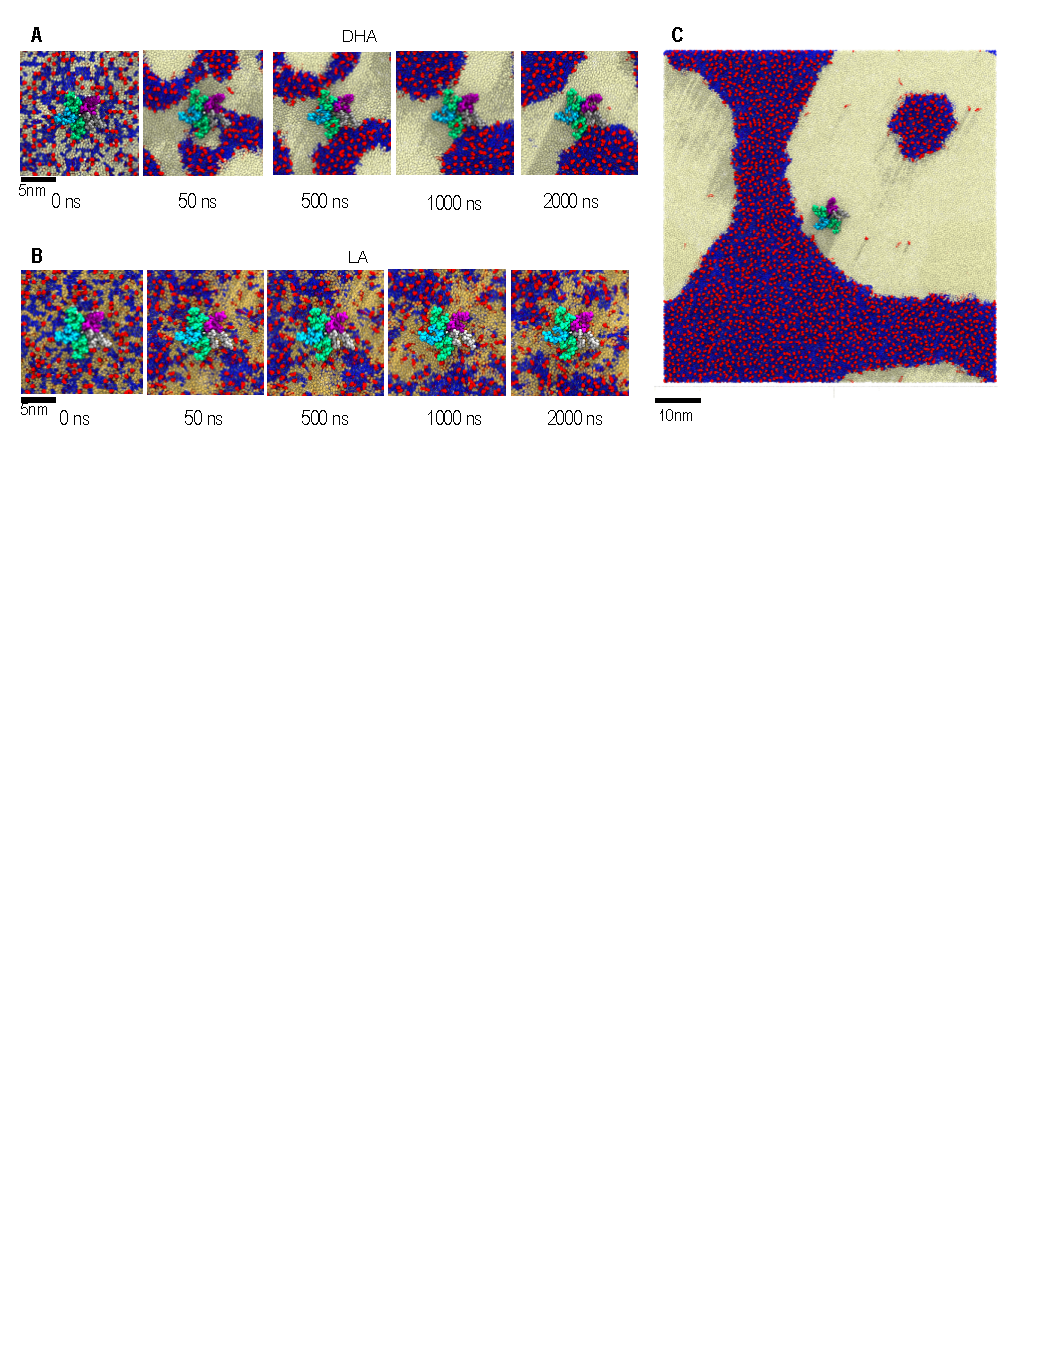
\includegraphics[width=1\linewidth]{Fig1.pdf}
		\caption{ Trajectories of ternary mixtures at ratios of 2:2:1 DPPC:PUFA:Chol. A and B: Trajectories of simulation systems with a single nAChR embedded within small membranes, using lipids containing DHA acyl chains or LA acyl chains. Both simulations were run for 2 $\mu$s. C: Final snapshot of 4 $\mu$s trajectory of a system within a large $\sim$ 75x75 nm$^2$ membrane with the same composition as in A. Subunits are colored: $\alpha$: green, $\beta$: purple, $\delta$: gray, $\gamma$: cyan. Lipids are colored: Chol: red, DPPC: blue, di-DHA-PE: white, DLiPC: tan.} 
		\label{fig:fig1}
	\end{figure*}

	\begin{figure}[!ht]
		\center
		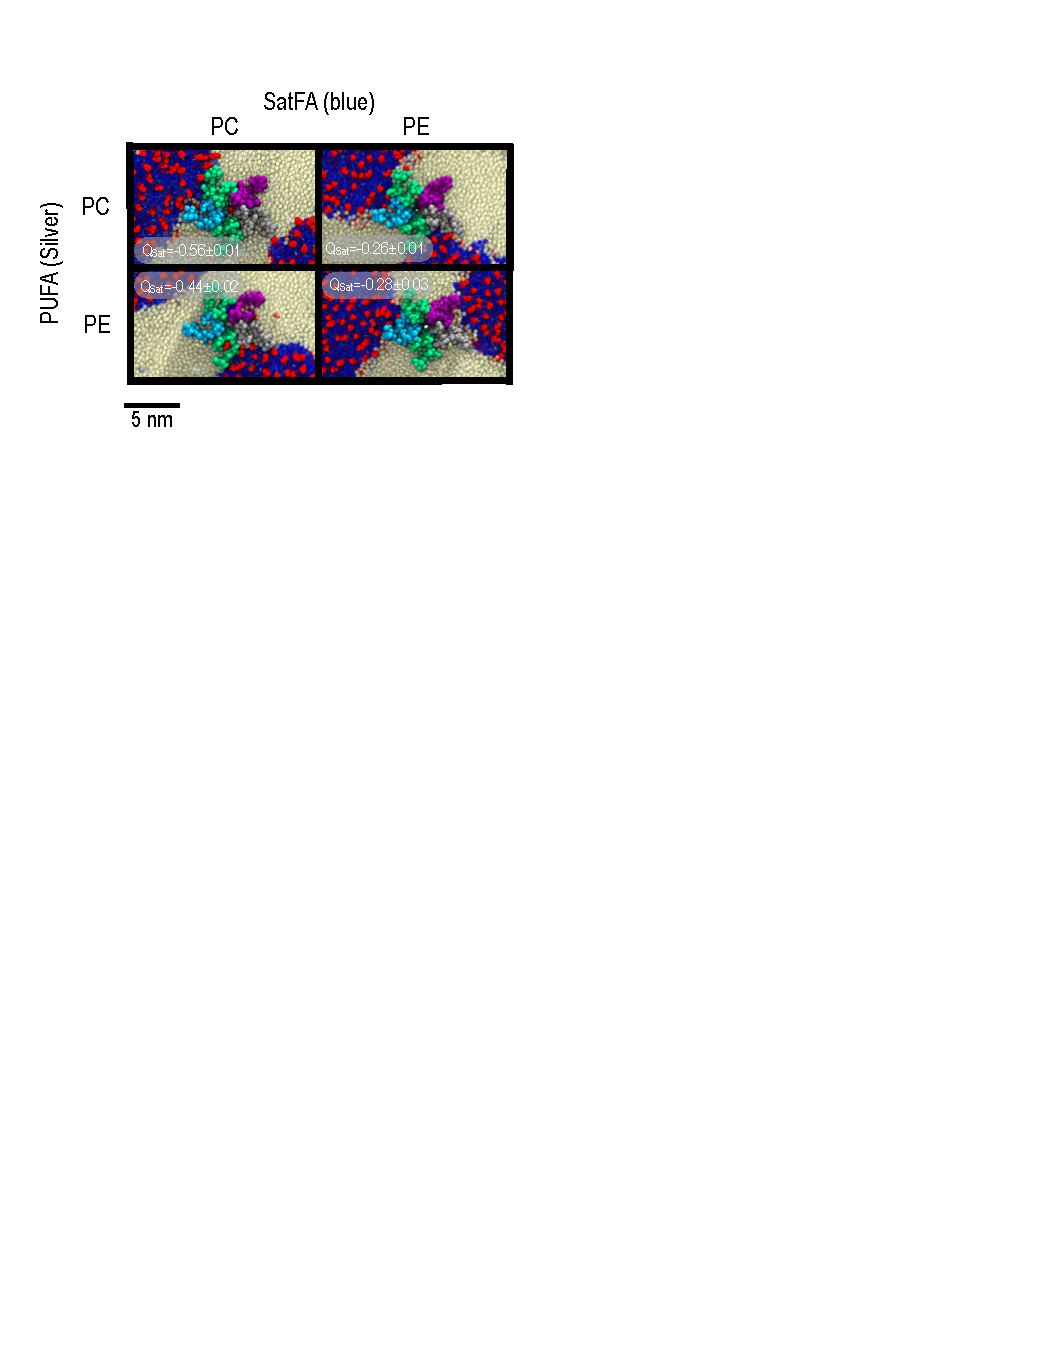
\includegraphics[width=1\linewidth]{SI_Q.pdf}
		\caption{ Comparison of nAChR partitioning based on lipid headgroups (PC and PE). All images represent last frame of 2$\mu$s  simulations of small membranes with composition  2:2:1 Sat:PUFA:Cholesterol.  Rows represent the head-group for the PUFA-containing lipid, while columns represent the head-group of the saturate lipid.   Each image includes $\qsat$ values related to individual systems with errors across averaging 50~ns blocks.}
		\label{fig:SIQ}
	\end{figure}
	%\liam{\cite{Parton2013,Goose2013,Scott2008}, which used multiple proteins assisted in membrane organization,
	%Since 
	%the single \nachr~molecule used within these experiments does not significantly affect membrane organization, which is instead driven by lipid-lipid interactions.} 
	
	The \nachr~annulus is highly enriched in DHA: DHA-PE constitute nearly 100\% of the local lipids even in membranes with very low DHA concentrations. This strong signal could indicate multiple high affinity sites for DHA chains across the transmembrane protein surface. At another extreme, DHA enrichment could be driven by a very slight preference for DHA in a highly non-ideal bulk: since DHA is found in well-defined domains without protein, even one DHA molecule that binds to the protein surface could stabilize the rest of the $\ldo$ domain nearby. Comparing boundary lipid and domain formation trends can help distinguish between these two scenarios.  If boundary lipid enrichment is determined purely by how well-defined domains are (the latter scenario), we would expect similar trends for $M_{DHA,DHA}$ and $Q_{sat}$ in the DHA column of Figure \ref{fig:fig2}.  In contrast,  Figure \ref{fig:fig2} shows that while domain formation in DHA-containing systems is only weakly sensitive to cholesterol content (horizontal contours), composition of boundary lipids is highly sensitive to cholesterol content (diagonal contours). These results suggest that direct interactions between multiple favorable sites on \nachr and DHA-containing lipids dominate the observed enrichment of DHA among boundary lipids.  
%	  In both randomly mixed binary systems (Figure \ref{fig:binary}B) and the partially-phase separated systems containing small amounts of LA (Figure \ref{fig:fig2}B, right), $\qsat$ is only weakly sensitive to cholesterol concentration. %,
	%with  
%	There is a slight amplification of saturated boundary lipid depletion as cholesterol is added and the saturated lipid is removed. This is consistent with the annulus of cholesterol in Figure \ref{fig:binary}C.   In highly phase-separated systems containing DHA, boundary lipid depletion decays as cholesterol is added, indicated by the diagonal contours in the DHA graph in Figure \ref{fig:fig2} B: for a given $\xunsat$, $\qsat$ increases with $\xch$.       %, suggesting that while saturated-\nachr~ interactions are unfavorable, \nachr-cholesterol interactions are favorable and saturated lipids are simply nearby.     This could indicate favorable displacement of saturated lipids by cholesterol in specific binding sites but not around the whole protein, or it could indicate  .  Saturated lipid depletion and cholesterol sensitivity was reduced in LA-containing mixtures,  as shown by the primarily horizontal contours in Figure \ref{fig:fig2} B.  
	%This could be consistent with cholesterol acting as a surfactant between \nachr~and a well-defined $\lo$ domain.    
	
	%The phase diagrams shown in Figure \ref{fig:fig2} compare the effects of two unsaturated lipids: DHA with a PE headgroup or LA with a PC headgroup.  
	The simulations represented in Figure \ref{fig:fig2} do compare the effects of two unsaturated lipids that also have different headgroups. DHA is far more commonly paired with PE in native membranes, while LA is more commonly found with PC. We found no qualitative differences in \nachr~domain partitioning or significant quantitative effect on $\qsat$ upon switching PC and PE headgroups on the PUFA lipid.  We did observe a quantitative effect of \emph{saturated} lipid headgroup on boundary lipid composition: $\qsat$ was reduced by half when saturated PE was used instead of saturated PC. (Figure \ref{fig:SIQ}).  As shown in Figure \ref{fig:SIQ}, \nachr~is bordered by $\lo$ domains on two opposing faces when saturated PE is used, compared to only one face if PC is used.  %(regardless of whether the PUFA has a PC or PE headgroup)
The particular domain topology shown in Figure \ref{fig:SIQ} is an artifact of the periodic boundary conditions, but still indicates more favorable interactions of \nachr~with an $\lo$ domain composed of DPPE vs DPPC. This may reflect a difference in the lipid shape (wedge-shaped DPPE vs cylindrical-shaped DPPC) and the associated monolayer spontaneous curvature.  For PUFA lipids in flexible $\ldo$ domains, lipid shape is less likely to play a significant role in determining partitioning. The dramatic difference in domain flexibility is apparent in  Figure SI \ref{fig:curve}.   %and the \nachr~ in the presence of DPPE is dependent upon shape of $\lo$ domain lipids, consistent with an interaction driven by elastic effects.  
	%, albeit not as critically for membranes including DLiPC.
	%\liam{Results do not vary using either of the zwiterionic head group}. 
	%A comparison of PC and PE head groups with C16:0 and DHA acyl chain preference is shown in . 
	%In all four figures nAChR resides in $\ldo$ phases, supporting of acyl-chain dependency over head-groups.
%	Trends for $\qsat$ \liam{across various ratios} of unsaturated lipid and cholesterol were highly sensitive to whether $n-3$ or $n-6$ lipids were used.  DPPC has such low affinity relative to $n-3$ lipids for most sites on the nAChR that $\bsat/\nbound  \le 10\%$ regardless of $x_{DPPC}$. Intermediate amounts of $n-3$ unsaturated lipids (between 30 and 40\%) further depletes DPPC from boundary lipids,  even over a wider range of cholesterol ratios.   
	
%	Figure \ref{fig:fig2}B shows boundary lipids are highly dependent on species of PUFA and cholesterol. Figure \ref{fig:fig2}B with DHA demonstrates an approximately constant $\qsat$ at cholesterol concentrations between $\sim$0.05\% to $\sim$25\%, maintaining $\sim$ constant DPPC concentration. $\qsat$ using the PUFA LA, still has a cholesterol dependence, however LA's affinity to mix with $\lo$ lipids maintains much higher values of $\qsat$. $\qsat$ values appear to be maximum in systems with near native $\xch$.
	
	\subsection{Spontaneous integration of lipids into nAChR TMD bundle} \label{Embed}

	The \nachr~structure used for these simulations was determined in a native membrane with a high fraction of polyunsaturated lipids. While we previously \cite{Brannigan_Embedded_2008} proposed that unresolved density in this structure could be embedded cholesterol, the possibility of occupation by phospholipids other than POPC was not investigated.  Furthermore, we did not consider possible asymmetry across subunits in binding previously.  Here we do observe penetration of both the intersubunit (``type B'') and the intrasubunit (``type A/C'') sites previously proposed, by both phospholipids and cholesterol, but with a high degree of subunit specificity.  
		
Two dimensional density distributions of DPPC, PUFAs, and cholesterol over short and long length scales were measured for two ternary mixtures and one binary mixture (Figure \ref{fig:sorting}).   In binary DPPC/cholesterol membranes, DPPC was more likely than cholesterol to occupy intrasubunit sites.  DPPC binds shallowly in the $\alpha$ subunit and more deeply in the $\beta$ subunit. Introducing PUFAs resulted in displacement of both cholesterol and DPPC from intrasubunit sites, except for the $\beta$ intrasubunit site, which became more likely to be occupied by cholesterol. The interior of the $\beta$ subunit TMD has the largest amount of available volume, could sequester cholesterol (but not DPPC) from the PUFA lipids in the annulus, and filling the interior with a PUFA chain may be entropically costly.  PUFA chains did occupy other intrasubunit sites, but remained fluid, as shown in Figure \ref{fig:sum}. 

	Intersubunit sites were rarely occupied by DPPC, with the exception of the $\beta+/\alpha-$ site in the binary system (Figure \ref{fig:sorting}). Intersubunit sites were more likely to bind cholesterol, particularly the $\beta+/\alpha-$, $\alpha+/\gamma-$, and $\alpha+/\delta-$ subunit interfaces. Occupation of $\alpha+/\delta-$ is consistent with cryo-EM observations\cite{Unwin_Segregation_2017}  of enhanced cholesterol density around the $\alpha+/\delta-$ site. Intersubunit sites that were not significantly occupied by cholesterol ($\delta+/\beta-$ and $\gamma-/\alpha+$) did show significant and deep occupation by DHA, which tended to enter from the adjacent intrasubunit site rather than from the membrane. Even those intersubunit sites with significant cholesterol occupancy can simultaneously bind part of a DHA chain, yielding non-vanishing DHA density.  
	
%	In both binary CHOL:SAT (Figure \ref{fig:binary} C) and ternary CHOL:SAT:PUFA mixtures (Figure \ref{fig:fig3}), phospholipid acyl chains are found at a high density in outer-ring embedded sites, farther from the pore, primarily in the center of the four helix bundles that comprise each subunit.  Comparison between these density plots indicates long chain PUFAs entirely displace saturated acyl chains found in this region in the CHOL:SAT systems.  DHA  also displaces cholesterol from these sites and some deeper intersubunit sites, consistent with its longer and more flexible acyl chains. Other intersubunit sites remain primarily occupied by cholesterol in these particular simulations, particularly $\beta+/\alpha-$ and $\delta+/\alpha-$. In ternary simulations with polyunsaturated lipids, cholesterol does still spontaneously occupy inter and intrasubunit gaps, but can be displaced by long polyunsaturated acyl chains.  

%	 Simulations also show cholesterol embedding within gaps of the 2BG9 cryo-EM structure \cite{Unwin_Refined_2005}, consistent with (see Figure \ref{fig:sum} sub-figure); \liam{ PUFAs occupied a substantial portion of nAChR} TMD (Figure \ref{fig:sum}).
%
%	\liam{To evaluate lipids embedding into nAChR}, we measured the average 2D density of lipids,  around the nAChR (Figures \ref{fig:binary} C and \ref{fig:fig3}). \liam{Figure \ref{fig:binary} measures the lipid density per a given bin $\rho$, equation \ref{eq:R}. DPPC and chol are shown interacting at the annular region, but cholesterol can embed into the protein as deep as the pore.}
%
%	\liam{Figure \ref{fig:fig3} DPPC is depleted from the protein, but PUFAs and cholesterol compete for gaps. We observe this trend to be more apparent in DHA than LA, and theorized it isdue to the greater degree of flexibility DHA acyl chains have has compared to LA acyl chains.}

	%\subsection{nAChR Preference for Domain Interface Including PUFAs} \label{Interface}

%	\subsection{Subunit selectivity of lipid interactions} \label{Interface}
%
%	\liam{With the inclusion of PUFAs, our simulations have consistently shown nAChR partitions into the $\ldo$ phase. Interestingly, nAChR is recurrently in close or direct contact with the $\lo$ phase for $23x23$ $nm^2$ membranes, imaged in Figure \ref{fig:fig1}A and C, Figure \ref{fig:SIQ}, oriented with $\alpha_{\gamma}/\gamma$ and $\delta/\alpha_{\delta}$ subunits having the greatest interaction with the interface. This is consistent with the results of \cite{Unwin_Segregation_2017}, who recently showed nAChRs $\delta$ subunit near a cholesterol enriched phase.} 
%
%	\liam{To test whether the proximity of the nAChR to the interface was simply due to the domain area to lipid number being small, the  membrane area was increased to $\sim 45x45$ $nm^2$; while nAChR comes into contact domain boundary or near the boundary in the larger system, it is more probable to remain in the $\ldo$ phase, showing no discernible subunit-lipid preferences.}
%	
%	%\liam{Comparatively, in small water boxes, nAChR shows $\lo$ interaction with $\alpha_{\gamma}$, $\gamma$, and $\delta$ subunits. Increasing the water box volume, however shows nAChR is uninterested in specific lipid-subunit interactions. Figure \ref{fig:fig3} column 1 shows significant depletion of DPPC, and enrichment of DHA making up boundary and annular lipids. In Figure \ref{fig:fig3} column 2, LA and cholesterol forms the boundary and annular lipids. There is a drop in DPPC concentration, but unlike column 1, DPPC remains quasi-mixed into the boundary lipids, with annular interactions at the $\alpha_{\delta}/\delta$ region.}
%
%	\liam{These results show, in ternary mixtures, nAChR with organizes the local membrane to be predominantly annular and non-annular PUFAs and a secondary density of cholesterol. Extrapolating this, nAChR may organize its local membrane similarly in complex membranes. A subunit-lipid preference is not readily observed in larger systems however.}
%
%	% This is consistent with the results of \cite{Unwin_Segregation_2017}, who recently showed partitioning of nAChR near a domain boundary using cryo-EM of nAChR in Torpedo electric organ membranes.}

	\subsection{Lipid sorting over the 5-20 nm range is associated with larger domains  } \label{Sorting}

	As shown in Figure \ref{fig:sorting}, observed sorting of lipids within {5-20~nm} of the \nachr~is dependent on the overall composition of the membrane. For all compositions shown, cholesterol is depleted within 5-20~nm and enriched far from the protein.  Within the binary systems this effect is minor ( $\tilde\rho_{CHOL} \sim 1$), but it becomes stronger in the moderately demixed LA systems ($\tilde\rho_{CHOL} \sim 0.5$) and substantial ($\tilde\rho_{CHOL} \sim 0.25$) for the highly-segregated DHA containing systems.  A similar pattern is observed for DPPC, which suggests that ``sorting'' over the 5-20~nm range is primarily driven by intrinsic differences in membrane organization that would be observed without the receptor. PUFAs are also most highly enriched at intermediate distances : the deepest red band is found at about 5~nm~in LA-containing systems and about 8~nm~ in DHA-containing systems.  This would be expected when \nachr~partitions near a curved domain boundary, as in Figure \ref{fig:SIQ}.      			
	 %\grace{?s want to know, about how far away from protein is darkest red band for PUFAs in Figure \ref{fig:sorting}}
		%\subsection {Subunit Preference} \label{Subunit} 

	%\liam{Evaluation of} whether different faces of the nAChR heteromer preferred to face different domains, we measured the average 2D density of lipids, \liam{with respect to membrane thickness,} around the nAChR (Figures \ref{fig:binary} C and \ref{fig:fig3}). \liam{Figure \ref{fig:binary} measures the lipid density per a given bin $\rho$, equation \ref{eq:R}. DPPC and cholesterol bound to the annular region indiscriminatingly.}

	%\liam{Comparatively, in small water boxes, nAChR shows $\lo$ interaction with $\alpha_{\gamma}$, $\gamma$, and $\delta$ subunits. Increasing the water box volume, however shows nAChR is uninterested in specific lipid-subunit interactions. Figure \ref{fig:fig3} column 1 shows significant depletion of DPPC, and enrichment of DHA making up boundary and annular lipids. In Figure \ref{fig:fig3} column 2, LA and cholesterol forms the boundary and annular lipids. There is a drop in DPPC concentration, but unlike column 1, DPPC remains quasi-mixed into the boundary lipids, with annular interactions at the $\alpha_{\delta}/\delta$ region.}

	%\liam{The system with LA (Figure \ref{fig:fig3} column 2) was observed to be mixed in comparison to column 1. LA is the dominant local lipid with cholesterol as close second. DPPC is not repelled from the protein, but as seen in column 1 there does appear to be a weak depletion shell around the annular region.}

	%%\liam{For all radial density plots a ''pin-wheeling'' effect is observed. This pin-wheeling is hypothesized as a potential result of the nAChR's periodic interactions with itself, deforming the membrane, however that has been inconclusive as of now. The pin-wheeling becomes less noticeable as the membrane surface area increases.}

	%\liam{These results show, in ternary mixtures, nAChR with organizes the local membrane to be predominantly annular and non-annular PUFAs and a secondary density of cholesterol. Extrapolating this, nAChR may organize its local membrane similarly in complex membranes. A subunit-lipid preference is not readily observed in larger systems however.}
	 %Comparing these figures \ref{fig:binary} C and \ref{fig:fig3} shows subunits showing preference for cholesterol (Figure \ref{fig:binary} C) have a preference for PUFAs (Figure \ref{fig:fig3}). 

	%%\liam{REMOVED: nAChR shows a preference for $\ldo$ domain between the $\alpha/\delta$ and $\beta/\alpha$ subunits, in ternary systems, is observed having greater preference for cholesterol in binary systems. This preference was not significant in the systems with the shorter, less flexible PUFAs.}

	%%\liam{Figure \ref{fig:fig3} shows a ''pinwheel'' pattern, that is consistent regardless of lipid species in ternary compositions. It is hypothesized this ''pinwheeling'' is a result of nAChR organizing the membrane. Conical proteins have been suggested to deform membranes, see \cite{Fournier2015}. Comparing \ref{fig:fig3} to \ref{fig:binary}, ''pinwheeling'' is only observed in the ternary membrane.}

	 %%$\rho_{DHA}$ depicts the $\alpha-/\gamma+$ subunits to have the greatest interactions with the $l_o$ domain(though $\alpha-/\delta+$ subunits have also shown strong interaction) , while the $\delta-/\beta+$ and $\beta-/\alpha+$ interfaces have greater preference for $\ldo$ domain. 

	

	%%Interestingly, cholesterol can weakly mix with the boundary shell, as observable in Figure \ref{fig:fig3}B. Cholesterol is  interacting with the DHA and the $\beta$ subunit, while remaining mostly randomly mixed with LA. In Figure \ref{fig:fig2}A, membranes lacking a protein promote more well defined domains, compared to membranes with embedded protein, suggesting nAChR assists in membrane organization to best support subunit-lipid affinity.



	%\liam{PUFAs lack embedding preferences. However cholesterol is consistently observed in the $\alpha_{\gamma}$, $\gamma$, and $\beta$ subunits (Figure \ref{fig:fig3}).}

	%%Figure \ref{fig:fig3} are heat maps showing the average density of lipid species ($\rho_a$) across three replicas. While DPPC is not observed to locally impact nAChR, DHA and LA are observed around the annular region and embedded throughout the protein, with preference for $\gamma$, $\delta$, and $\beta$ subunits. Interestingly, cholesterol is frequently seen in $\gamma$, $\delta$, and $\beta$ subunits, the same as the PUFAs used, though cholesterol does not readily mix with unsaturated lipid species.

	%%PUFA-cholesterol TMD occupation can more readily be observed in Figure \ref{fig:sum}. A late trajectory snap-shot showing cholesterol and DHA penetrating through out nACHR.  In this simulation,  DHA distributed through out most of the protein, with cholesterol embedding through $\alpha$, $\beta$, and $\delta$ subunits.

	%DHA and cholesterol are observed embedding frequently, see Figure \ref{fig:fig3} \textbf{a left}. In a number of cases, lipids may embed as deep as the pore. Figure \ref{fig:fig3}a right shows DLiPC and cholesterol to embed throughout the protein. LA binding within the pore is not as common as it is with the DHA acyl chain. DPPC is not observed to frequently bind beyond the annular region of the protein.s

	\begin{figure*}[h]
		\center
		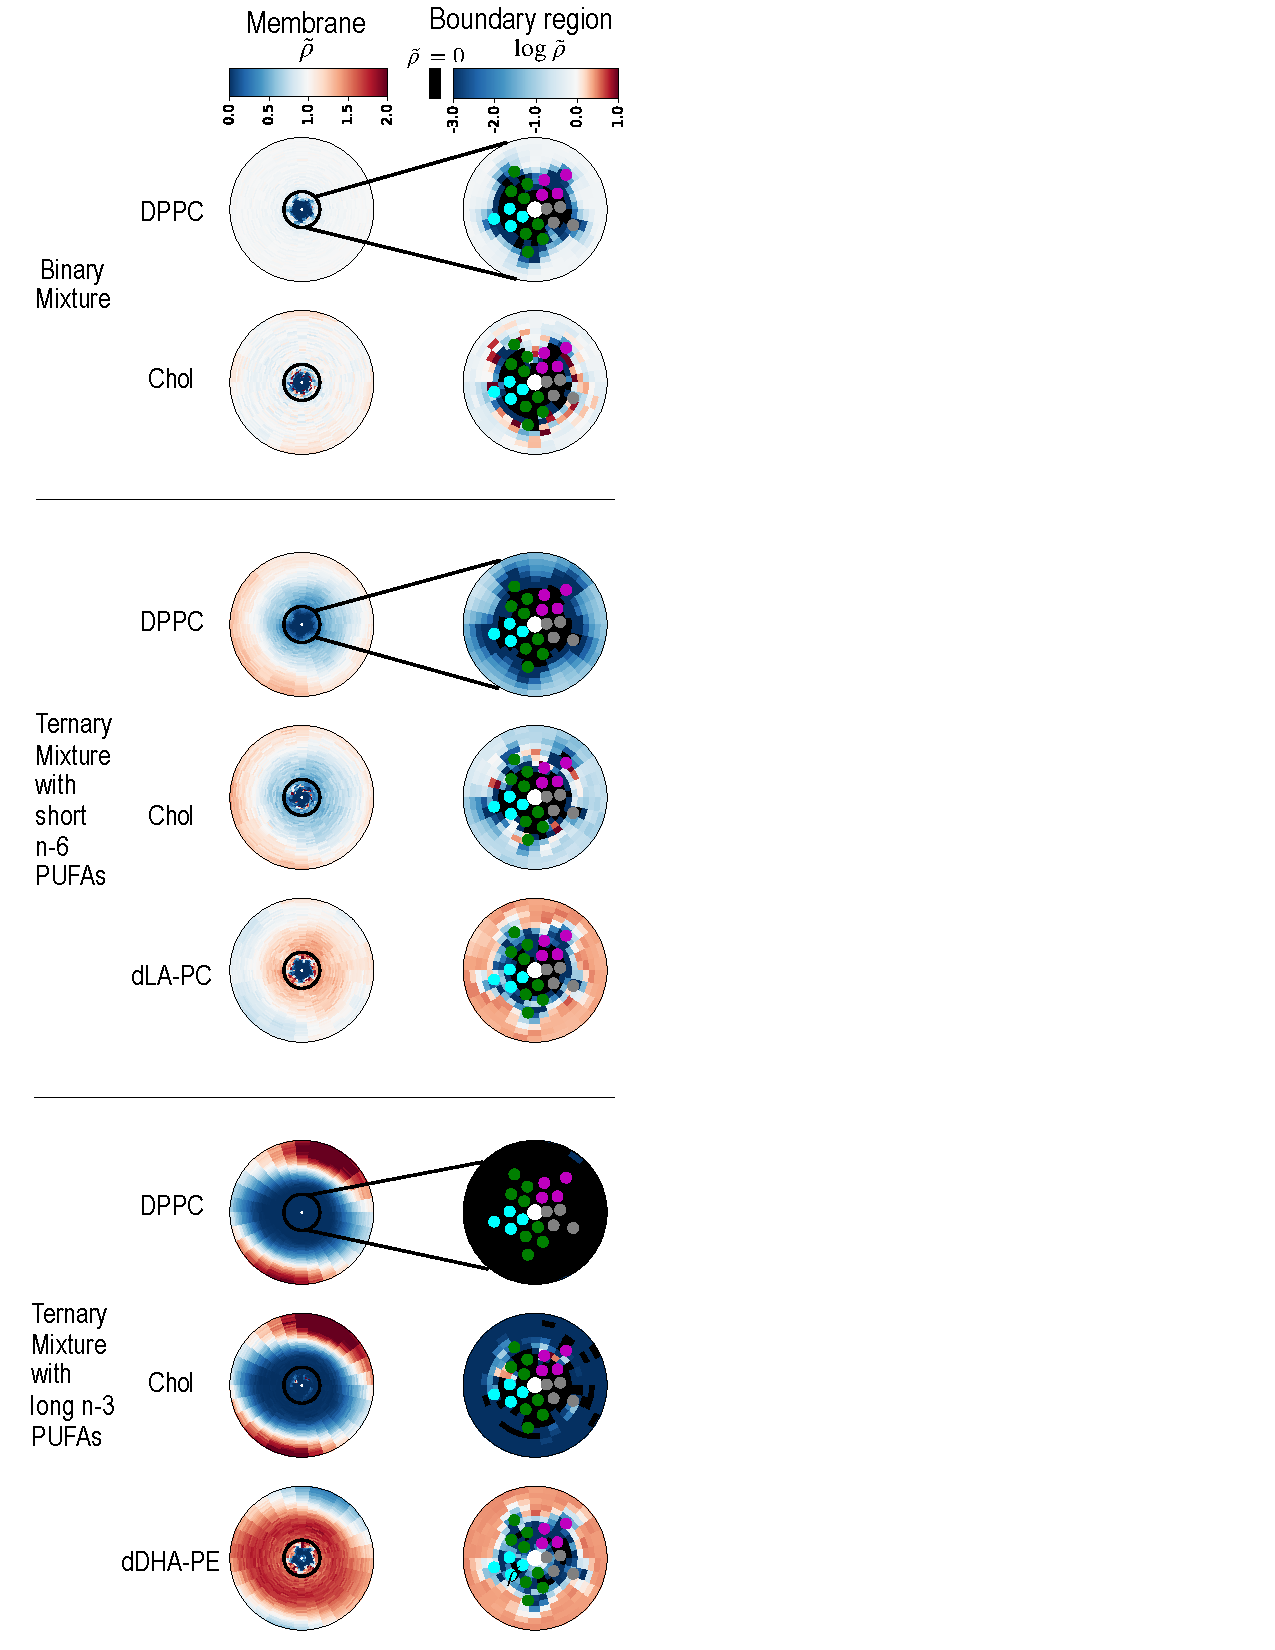
\includegraphics[width=1\linewidth]{ComparativeHeatMap.pdf}
		\caption{\liam{(left) Lipid distribution at long length scales. (right) Lipid bead distribution local to the nAChR TMD helices.} (Left) Heat maps representing normalized average lipid density are calculated over the last half of a $10 \mu$s simulation with composition DPPC:PUFA:CHOL 2:2:1 (as in Figure \ref{fig:fig1}A and B)  or  DPPC:CHOL 4:1 (as in Figure \ref{fig:binary} A and C) . ${\tilde{\rho}}_{a}$ is normalized by expected density based on composition (defined in eq \ref{eq:Rt}); white indicates no enrichment or depletion. \liam{The circle at the center of each heat map represents the right side figures. These heat maps to not include the \nachr~subunits plotted.}  (Right) Data is identical to the left figure but colorscale is adjusted and logarithmic density is shown, for representation of specific lipid binding. All beads for each lipid were used to calculate the density distribution, and density was normalized by expectation based on composition and number of beads per molecule.  Bins in which no density for the given lipid type was detected are shown as black.  Circles represent nAChR TMD helices, colored by subunit as in Fig. \ref{fig:binary} A.\grace{Update caption once figure is finalized}}
		\label{fig:sorting}
	\end{figure*}

	%\begin{figure}[h!]
%		\center
%		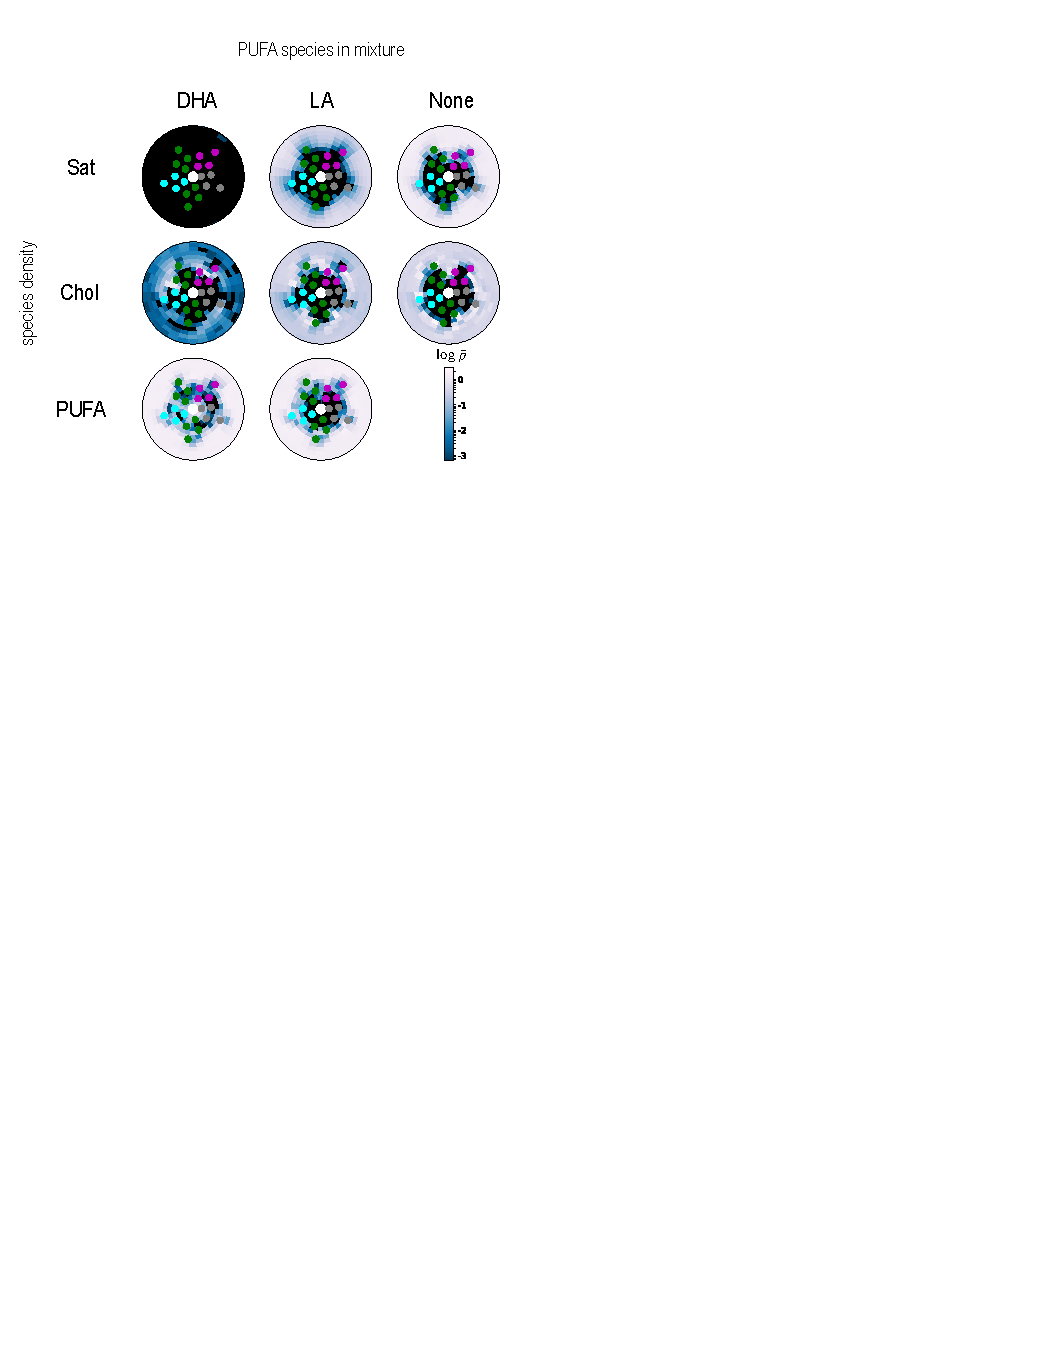
\includegraphics[width=1\linewidth]{Fig3.pdf}%
%		\caption{Lipid bead distribution local to the nAChR TMD helices. Data is identical to Fig. \ref{fig:sorting} but colorscale is adjusted and logarithmic density is shown, for representation of specific lipid binding. All beads for each lipid were used to calculate the density distribution, and density was normalized by expectation based on composition and number of beads per molecule.  Bins in which no density for the given lipid type was detected are shown as black.  Circles represent nAChR TMD helices, colored by subunit as in Fig. \ref{fig:binary} A. } 
%		\label{fig:fig3}
%	\end{figure}
	%Heat maps in Figure \ref{fig:fig3} \textbf{b} show the average density of cholesterol $(\rho_{Chol})$ within a membrane. $\rho$ is generally defined by equation \ref{eq:R}. In \ref{fig:fig3}b left, the system has a composition DHA-PE:DPPC:Chol 40:40:20. Chol is found in the $l_o$ domain. However, while $\beta$ subunit is partitioned into the $l_d$ phase, there is significant increase in $\rho_{Chol}$ within the $\beta$ subunit. In \ref{fig:fig3} \textbf{b right} DLiPC:DPPC:Chol 40:40:20, $\rho_{Chol}$ is greatest throughout the protein, with largest value within $\delta$ subunit.

	%Figure \ref{fig:fig3} shows the average of three replicas of PUFA:DPPC:Chol 40:40:20, where the PUFA is either DHA-PE or DLiPC. Protein chain locations are also averaged, resulting in a compressed area. Cholesterol is still observed to partition near or within nAChR and in the $l_o$ phase in systems containing DHA. It is highly dispersed within the bulk membrane and embedded with nAChR in systems with DLiPC. Saturated lipids in both series of systems tend to form the bulk membrane, and do not readily interact with nAChR. PUFAs tend form a dense boundary area around nAChR. Chol is observed to embed within or between subunits indiscriminately.

	\begin{figure}[h!]
		\center
		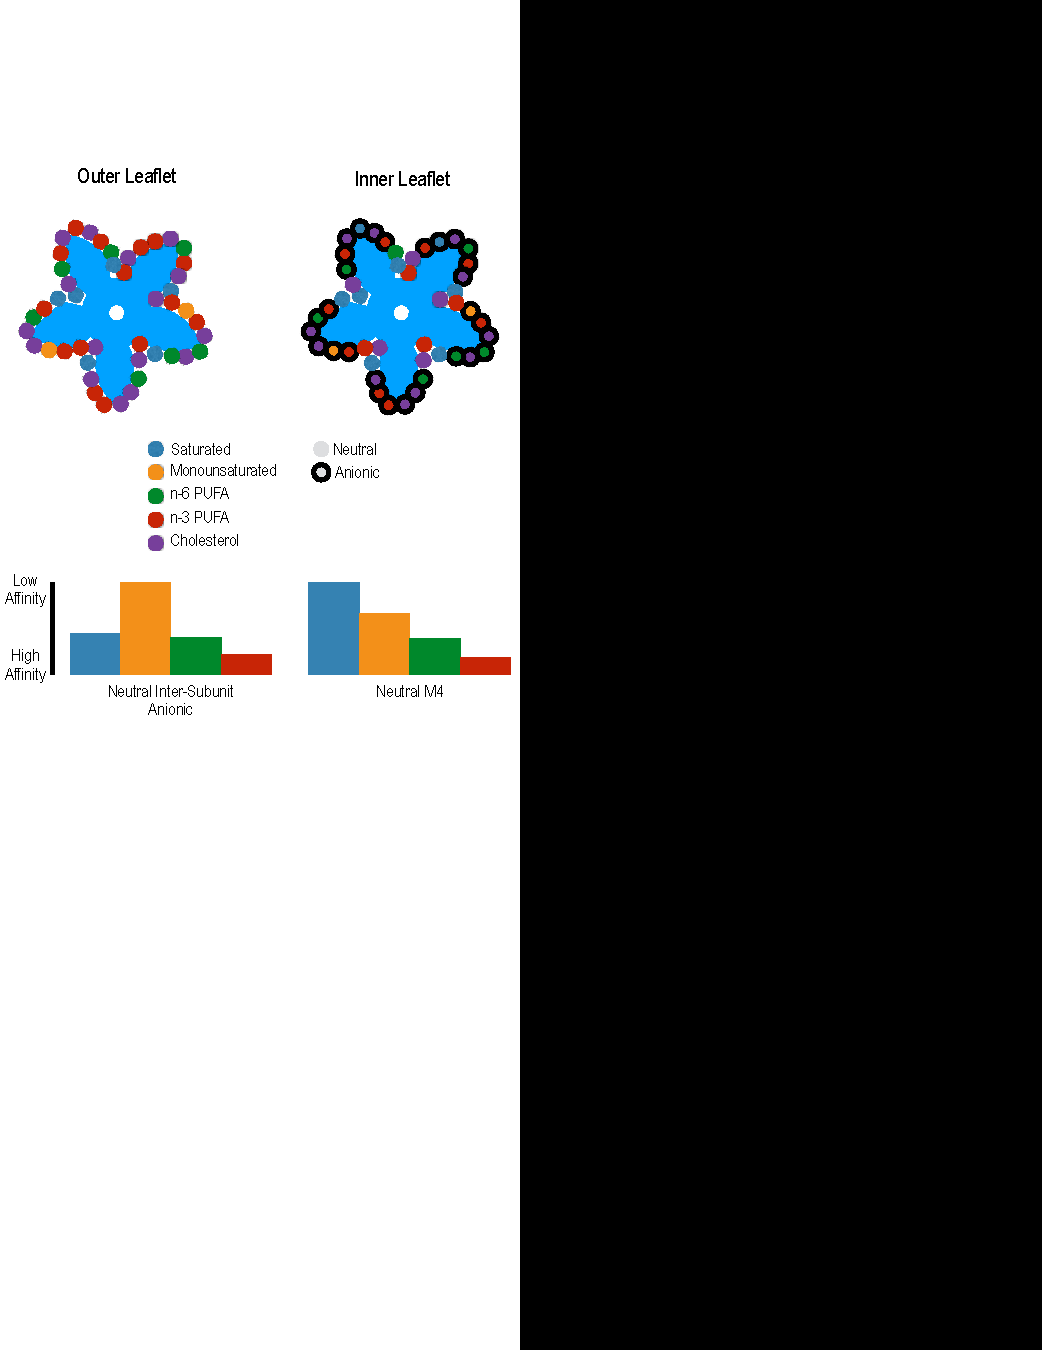
\includegraphics[width=1\linewidth]{Summary.pdf}
		\caption{ Embedded lipids in the nAChR. Main image: Representative frame from equilibrated small membrane simulation of nAChR in 2:2:1 DPPC:DHA-PE:CHOL. Backbone beads of the TMD helices are colored by subunit as in Figure \ref{fig:fig2}; side-chain beads are not shown.  Both DHA-PE (white) and cholesterol (red) equilibrate to embedded sites in the subunit center and subunit interfaces, although most cholesterol is found in the $\lo$ phase with DPPC (blue). Inset : Cryo-EM density of nAChR from \cite{Miyazawa2003} as rendered in \cite{Brannigan_Embedded_2008}; dark blue indicates high density, white is medium density, and red is low density. } 
		\label{fig:sum}
	\end{figure}

	 

\section{Aims of the PhD Proposal}
\input{../../Manuscripts/nAChR_2BG9_ModelMembrane_Liam/Letter_2017/Lipid_Tabel}
\subsection{Aim 1: Coarse-grained simulations of multiple subtypes of mammalian pLGICs in quasi-physiological membranes}
\begin{figure}[t!]\center
	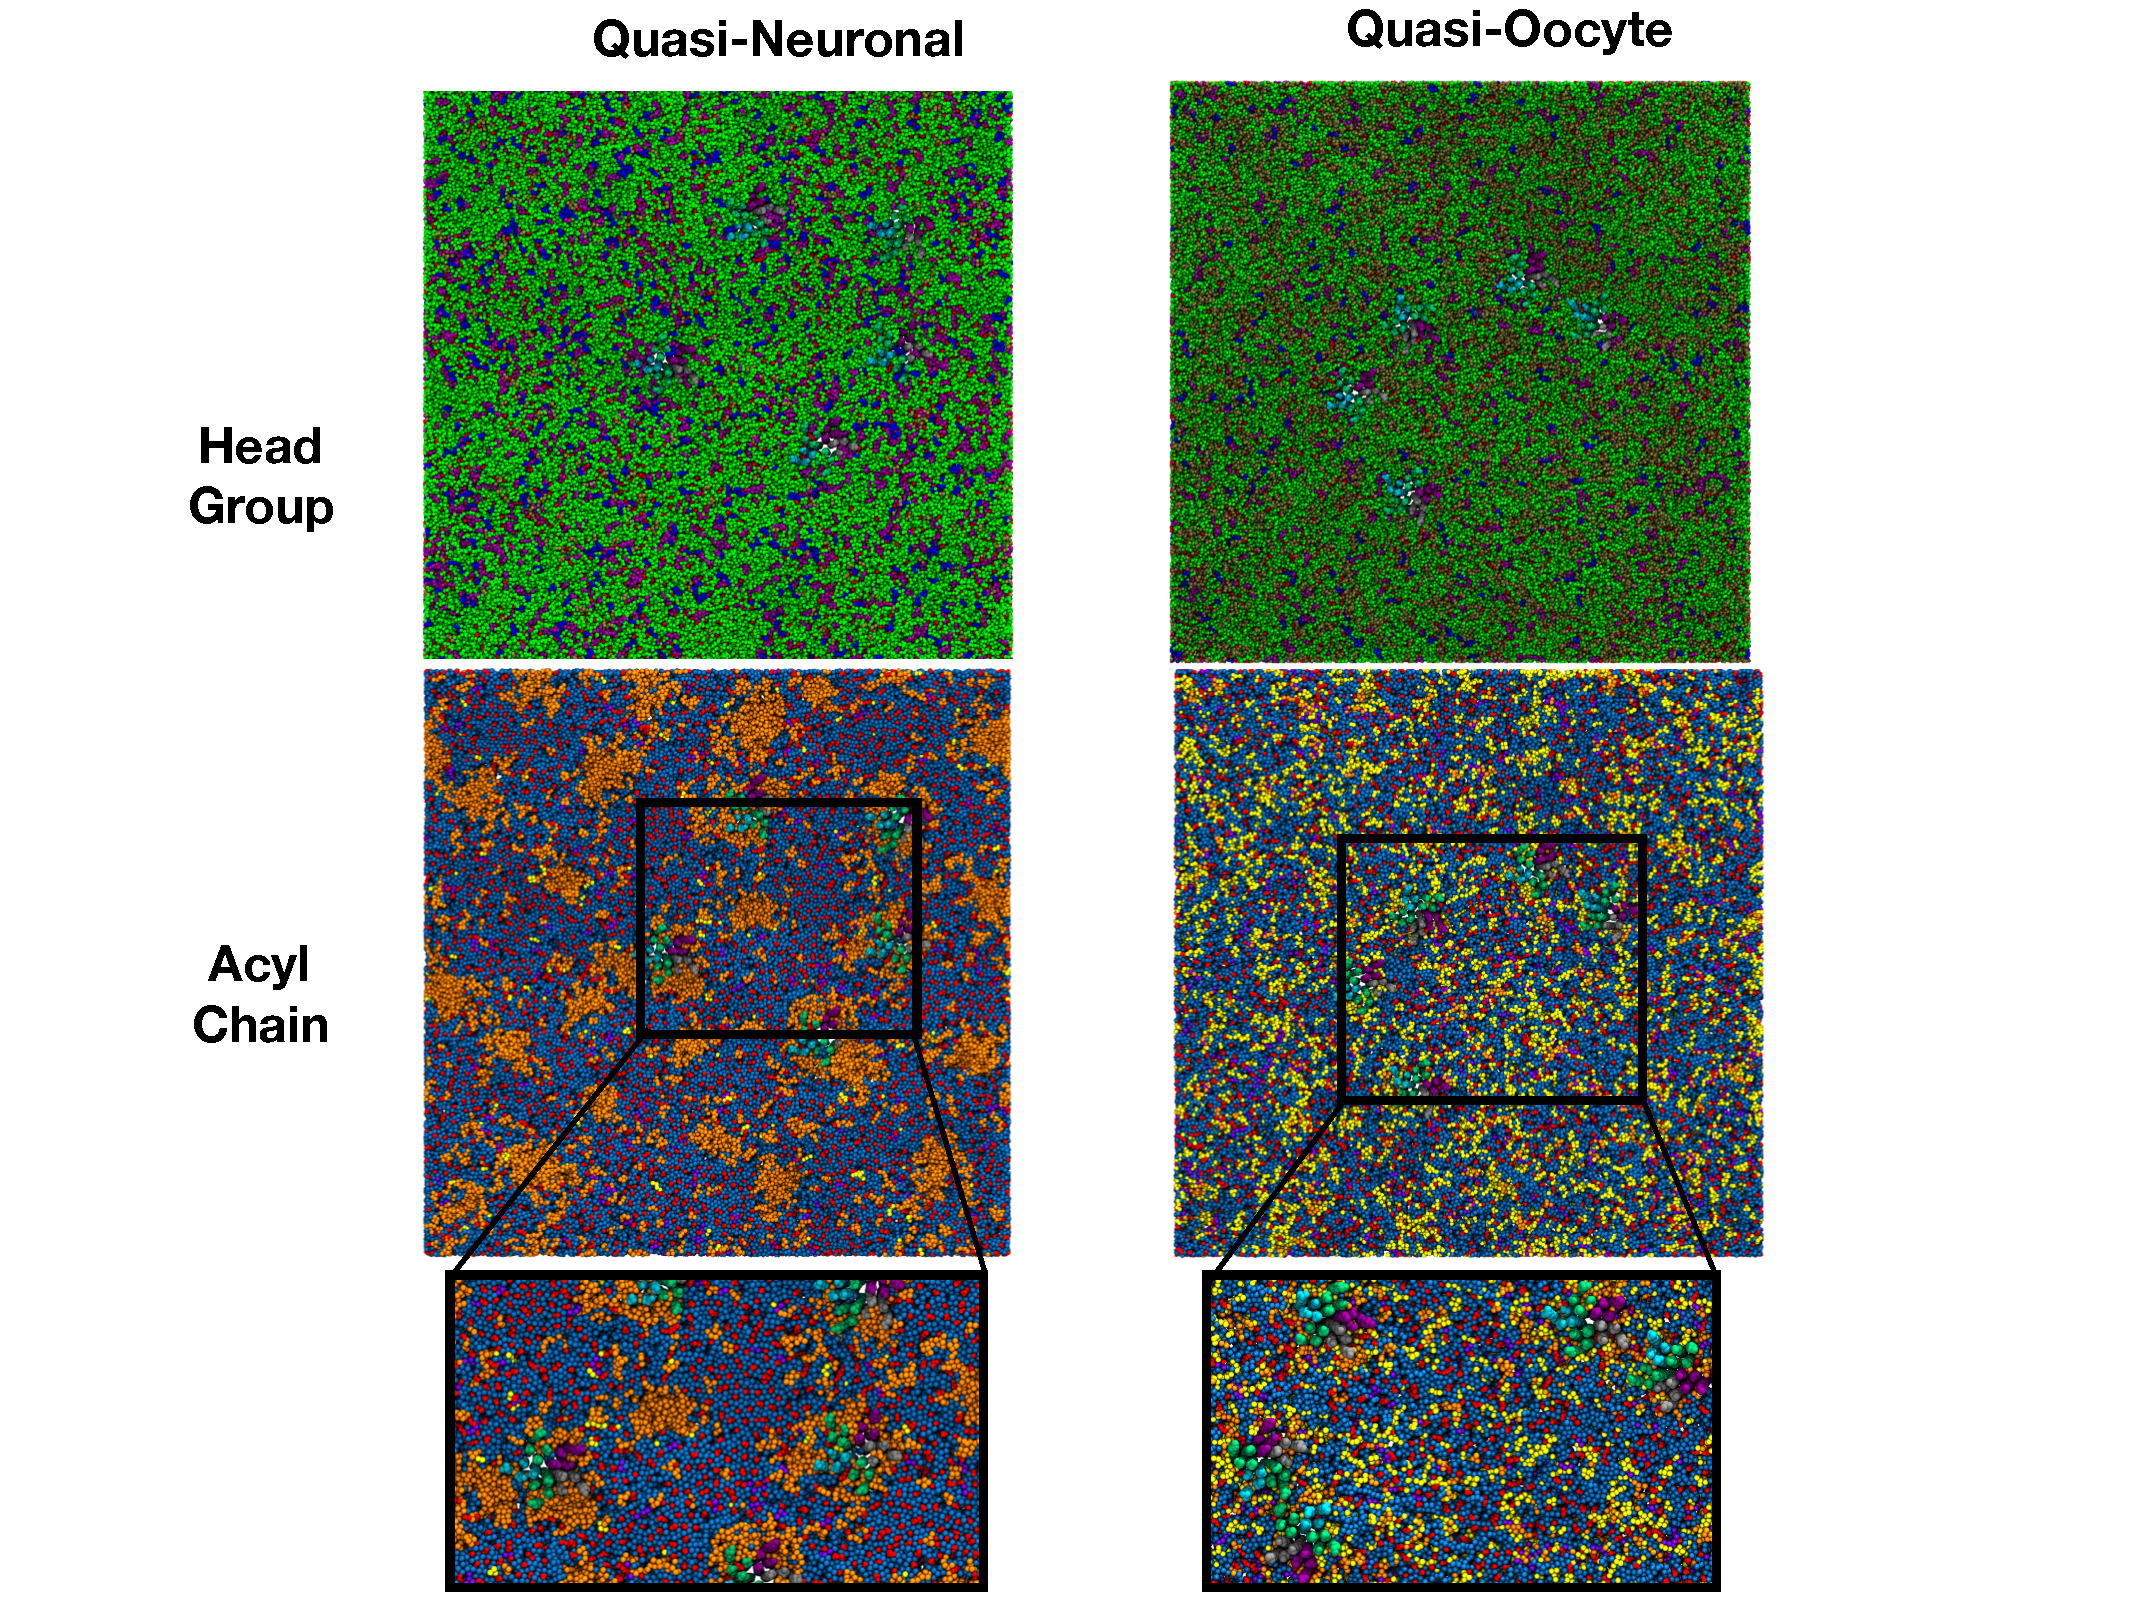
\includegraphics[width=1\linewidth]{./Images/Memb_Comp.pdf}
	\caption{Comparison of nAChR lipid sorting in quasi-Neuronal and quasi-Xenopus oocyte membranes, colored according to either phospholipid head-group or location of acyl chain unsaturation, from coarse-grained MD simulations. nAChR transmembrane domain is shown in surface representation, colored by subunit. Top row: PE (purple), PC (green), SM (tan), PS (blue), cholesterol (red). Bottom Row: n-3 (white), n-6 (yellow), n-9 (purple), saturated (blue), cholesterol (red). Composition of quasi-Neuronal and quasi-Oocyte membranes reflects all species that are sufficiently abundant to yield at least 2 molecules in a membrane of the simulated size. Both systems are fun for $\sim$ 1.5 $\mu s$}
	\label{fig:ooct}
\end{figure}

We observe nAChR partitioning into  n-3 polyunsaturated fatty acid (PUFA)  rich domains with the n-3 PUFA DHA-PE as nAChR's primary boundary lipid. The concentration of n-3 lipids is much lower in membranes, such as Xenopus oocytes,  commonly used in electrophysiology experiments, than in native membranes. I hypothesize adding small concentrations of n-3 is likely to restore the native boundary lipids. I will model various n-3 supplemented quasi-physiological membranes (such as oocytes) to predict those likely to provide a native local environment within the non-native membrane.

pLGICs have complex gating behavior and structural requirements, and nAChRs are some of the most complex pLGICs. One of the most poorly understood components of nAChR is its unpredictable functional sensitivity to slight changes in its lipid environment, a property shared to a lesser extent by other pLGICs \cite{M.CriadoH.Eibl1982,Conti2013}.

Considerable experimental effort \cite{Fong_Correlation_1986,Sunshine_Lipid_1992,Hamouda_Assessing_2006,Butler_FTIR_1993,Bhushan_Correlation_1993,Fong_Stabilization_1987,Corrie_Lipid_2002} was expended, primarily in the 1980s and 1990s, to understand the underlying mechanism of nAChR lipid sensitivity, including identifying the likelihood of specific boundary lipids. Experimental studies focused primarily on cholesterol, which were required in native membranes (20-40\% of lipid composition) to support native levels of ion flux in purified and reconstituted nAChR \cite{Fong_Correlation_1986,Fong_Stabilization_1987}. Further experiments showed that while cholesterol could be depleted from the bulk membrane, a second pool of cholesterol could not be removed from nAChR-containing membranes by depletion \cite{Leibel1987}. However, results were inconclusive regarding whether cholesterol was sufficient to restore nAChR function. Interestingly, soybean lipids (which are also high in n-3 PUFAs) \cite{Yoshida1986,Regost2003,Olsen2003} are more effective at restoring ion flux than cholesterol alone \cite{Morales2006}.

%\begin{figure}[t!]\center
%	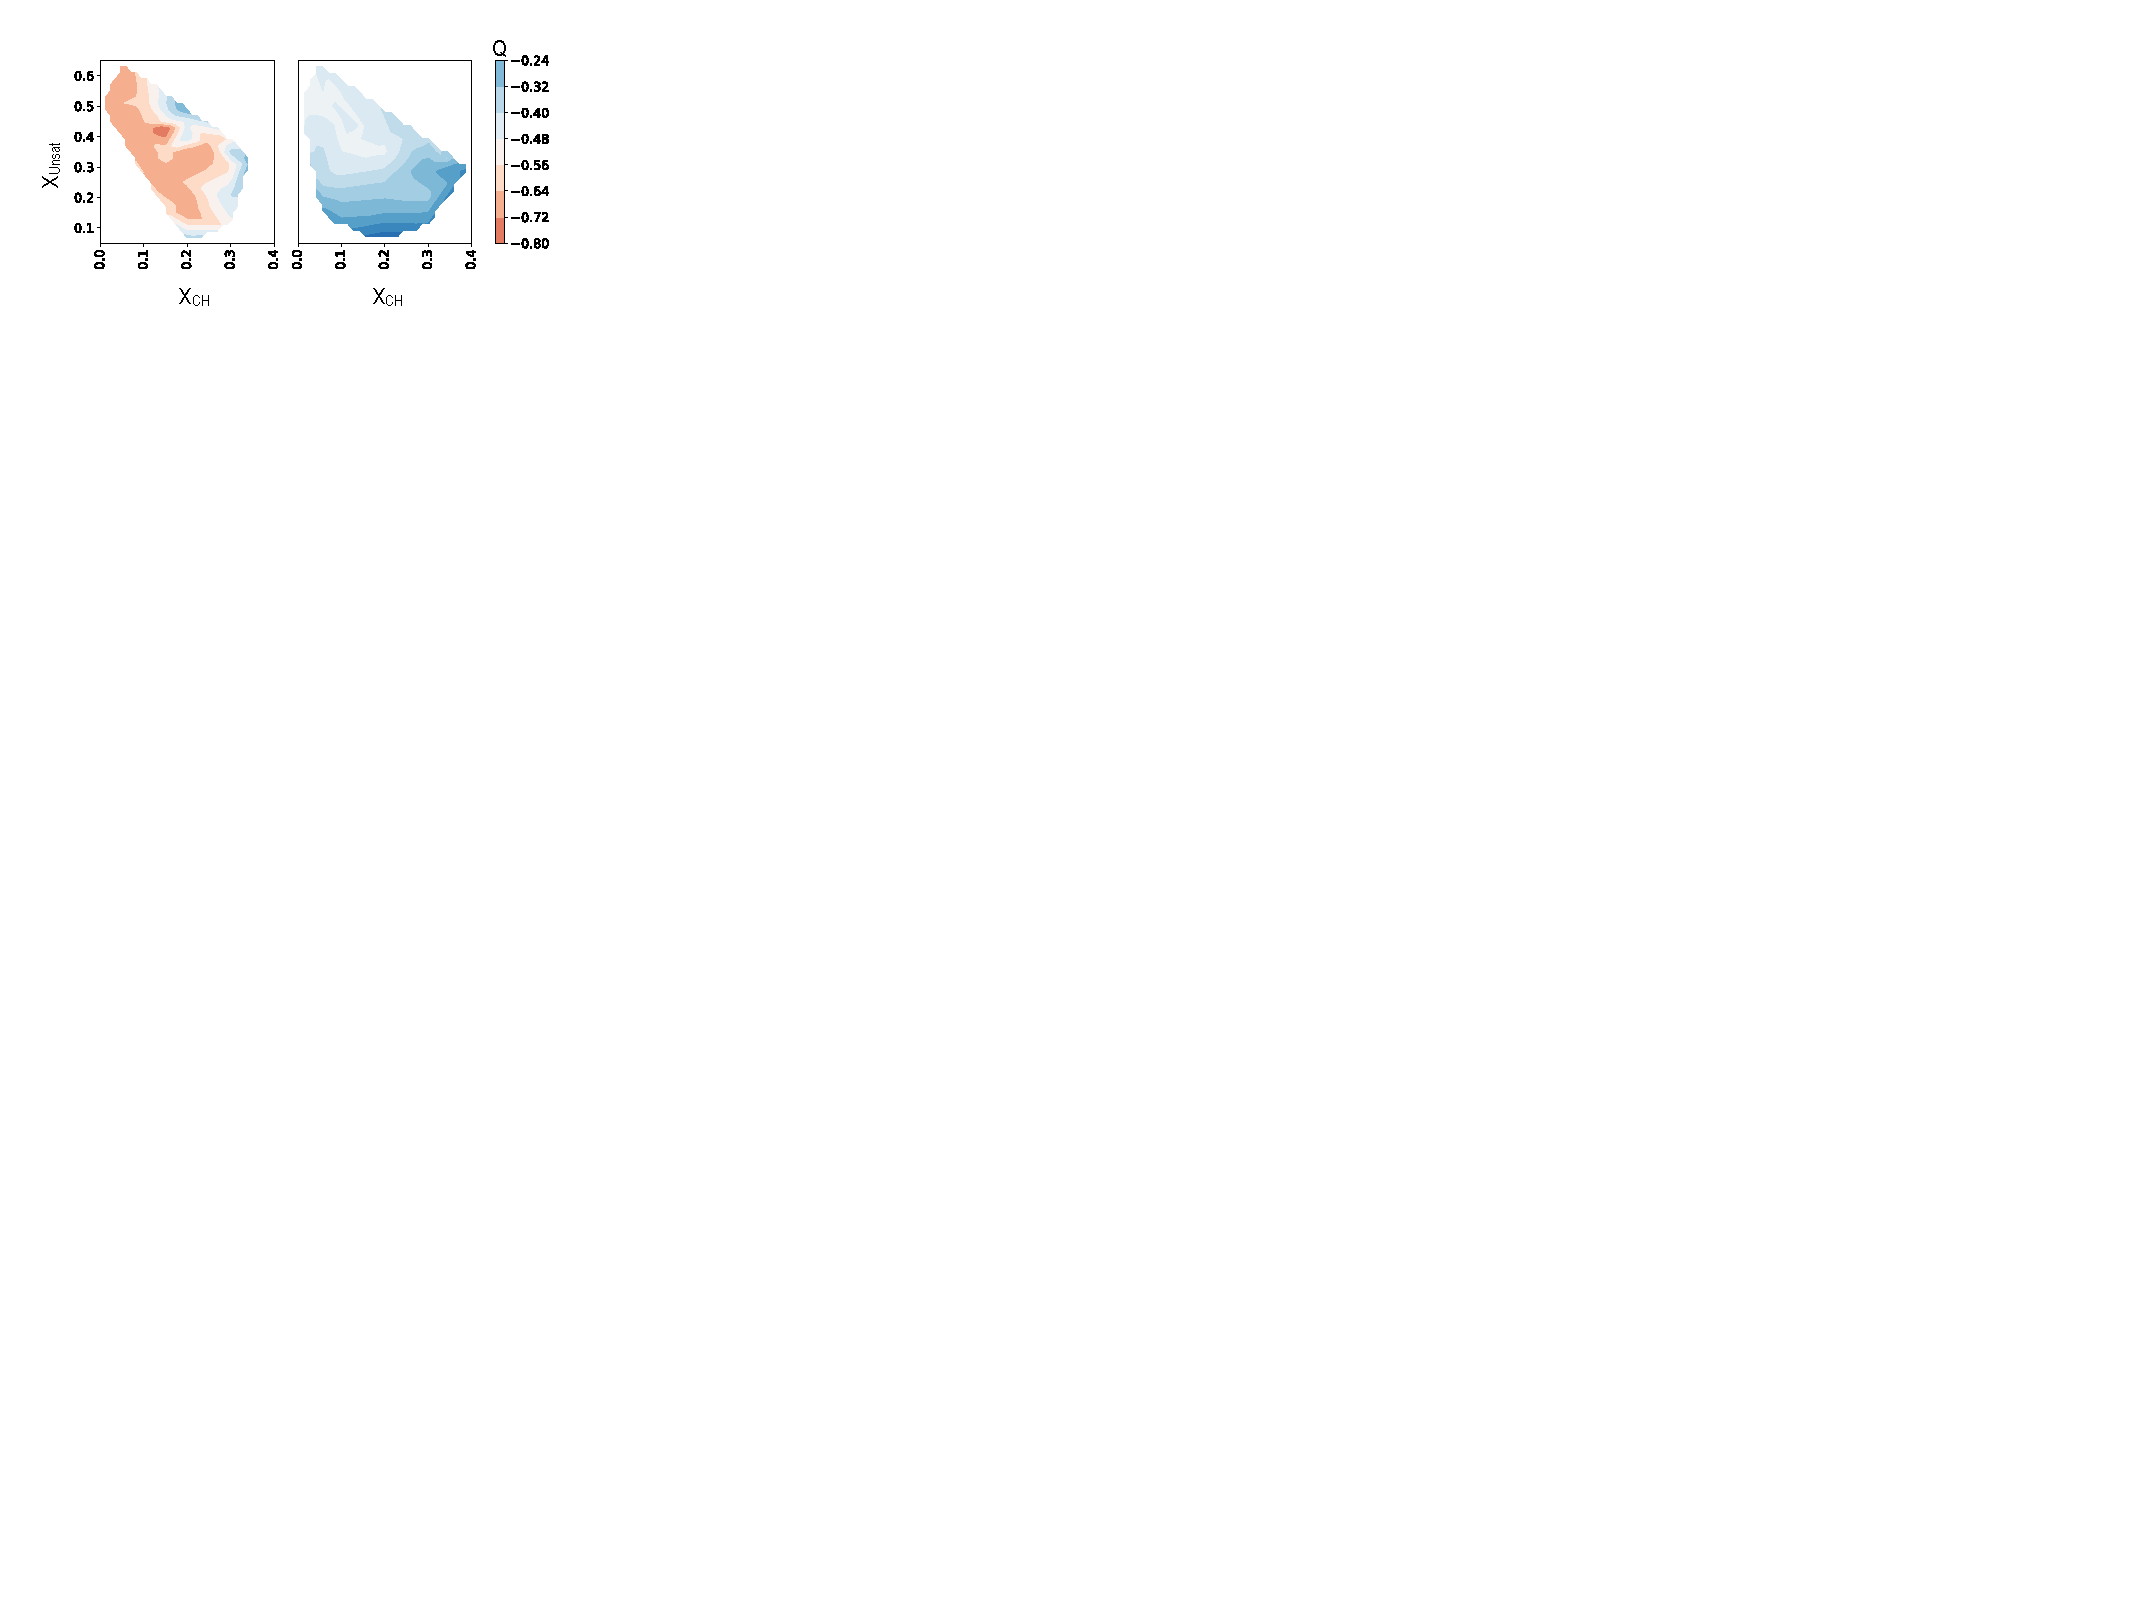
\includegraphics[width=1\linewidth]{./F31/Q.pdf}
%	\caption{Enrichment of nAChR annular lipids for saturated phospholipids in ternary mixture of cholesterol, saturated, and unsaturated phospholipids. $\qsat\equiv \frac{1}{\xsat}\left\langle\frac{  \bsat }{\nbound }\right\rangle-1$, where $\langle bsat\rangle_{\nbound}$ is the averaged fraction of boundary lipids composed of saturated phospholipids, $N_B$ is the total number of boundary lipids, and $\xsat$ is the bulk mole fraction of saturated phospholipid chains. $Q>0$ indicates nAChR preference for the $l_o$ domain; $Q<0$ indicates nAChR preference for the $l_{do}$ domain.}
%	\label{fig:Q}
%\end{figure}

The working assumption in the time of most of those experiments was that the membrane was randomly mixed in the absence of protein, although lipid sorting by proteins was considered likely; there was little evidence available then that cholesterol by itself can induce non-random mixing and even domain formation in just a ternary lipid mixture. We are now also aware of the critical role of acyl chain unsaturation in this process, but previous experiments focused primarily on the role of cholesterol and phospholipid headgroup without including the lipids with n-3 PUFA chains that are so abundant in both the fish electric organ and the postsynaptic membrane.

It is still unknown what factors determine the lipids interacting directly with pLGICs , leading to a substantial source of uncertainty in present-day experiments and introducing a divergence between simulations and experiments that cannot be reasonably estimated. Ionic flux of reconstituted neuronal $\alpha$3$\beta$4nAChR expressed in Xenopus oocytes is less than 50\% of those expressed in mouse-fibroblasts, with neither consistently reproducing native behavior \cite{Fong_Correlation_1986,Sunshine_Lipid_1992,Hamouda_Assessing_2006,Butler_FTIR_1993,Bhushan_Correlation_1993,Fong_Stabilization_1987,Bednarczyk_Transmembrane_2002,Corrie_Lipid_2002}. Contrasts in membrane lipids may contribute significantly to these differences, and specific lipid incorporation may bypass the need for microtransplantation of entire sections of neuronal membranes \cite{Conti2013} into oocytes to achieve native function.
%It is still unknown what factors determine the lipids interacting directly with pLGICs , leading to a substantial source of uncertainty in present-day experiments and introducing a disparity between simulations and experiments that cannot be reasonably estimated. Conductance of recombinant neuronal a3b4nAChR expressed in Xenopus oocytes is less than 50\% of those expressed in mouse-fibroblasts, with neither consistently reproducing native behavior. [34] Differences in membrane lipids may contribute significantly to these differences, and rational lipid supplementation may forgo the need for microtransplantation of entire sections of neuronal membranes[35] into oocytes to achieve native function.

%\subsubsection{Innovation}

A large number of experiments, ranging from the straightforward to the particularly sophisticated, have been carried out to investigate the mechanisms underlying cholesterol modulation of pLGICs. The proposed studies involve investigation of lipid interactions with nAChR via coarse grained molecular dynamics. Numerous simulations of nAChR and other pLGICs with atomic resolution, powerful methods for investigating direct interactions of receptors with small molecules, are also reported in the literature. In the absence of realistic estimates for the protein-local lipid composition, most such simulations embed the receptor in a model membrane composed of DOPC or POPC, with occasional inclusion of cholesterol.

My preliminary studies, which use CG simulations capable of equilibrating a quasi-native membrane, indicate that nAChR has a surprisingly strong preference for n-3 PUFAs (Figures \ref{fig:ooct} and \ref{fig:fig2}B) as boundary lipids. Although these lipids are abundant in most native nAChR membranes, including the electric organ, they had not been included in experiments (except via an abundance in soybean lipids). This surprising observation, if true, offers possible explanations for limited success of many previous experiments.

It further suggests that regardless of the bulk membrane composition, nAChR functions natively in a homogeneous local environment of n-3 PUFAs. Our proposal for reproducing native boundary lipids within an oocyte relies on both this simplicity and the large difference in abundance of n-3 PUFAs between the oocyte and the neuron, which suggests there is a qualitative difference in lipid environment. Microtransplantation of neuronal cell membranes into oocytes \cite{Conti2013} has been carried out and shown to improve ion flux through nAChRs embedded in oocyte membranes, but I will run calculations to inform an approach which restricts supplementation to a few species of preferred boundary lipid, and would substantially improves experimental control. These predictions will be tested by a collaborator of Dr. Brannigan’s, Dr. John Baenziger at University of Ottawa.

%\subsubsection{Approach}

I propose a series of simulations characterizing the boundary lipids surrounding nAChR embedded within a modified oocyte membrane, with the aim of finding the modifications which will reproduce native boundary lipids. %Our initial simulation results suggests nAChR partitions into $l_{do}$ with long chained PUFAs as boundary lipids (see Figure \ref{fig:ooct} and \ref{fig:fig2}B).

The proposed simulations will involve quasi-Oocyte lipid membranes and supplementing them with boundary lipids found in neuronal membranes. I will, first perform literature searches prudent to neuronal/synaptic, \textit{Xenopus} oocyte, and \textit{Torpedo} electric organ membrane compositions. If detailed compositions are not available, I will construct an acyl chain to acyl chain randomizer, to cover all potential lipid species. Constructing a spread sheet (Microsoft Excel) or program (in python), compare and select appropriate Martini equivalent lipids, based on acyl chain length and saturation. Having built a complementary selection of lipids, I will implement automation to allow for easy lipid to membrane supplementation. As there are various n-3 PUFAs, I will construct various series to test which neuronal/\textit{Torpede} n-3 lipid species best assist with native like nAChR boundary domains.

%Differences in the local lipid environments surrounding pLGIC when expressed in common lines for cultured cells will be obtained by computational microscopy; embedding nAChRs in membranes approximating various cell lines including post-synaptic membranes, and \textit{Xenopus} oocytes \cite{Lindi2001,Gamba2005}. 

It is possible (especially if elastic effects are essential) that increasing the number of receptors or the system size will modify these distributions. It is important then, to increase the number of receptors (aiming at around ten), enforcing realistic leaflet asymmetry, and incorporating the newer $\alpha$4$\beta$2 nAChR structure \cite{Morales-Perez_X_2016}. 
%Must be a better way to write this..
%Differences in the local  environment of the pLGIC when expressed in common lines for cultured cells will be obtained by computational microscopy of nAChRs in membranes approximating native membranes, including post-synaptic membranes, as well as common expression systems including Xenopus oocytes[57]. 

%It is possible (especially if elastic effects are essential) that increasing the number of receptors or the system size will modify these distributions. %Therefore, the first step of this aim is improving realism of the simulations of nAChR in the neuronal membrane,
%It is important then, to increase the number of receptors (aiming at around ten), enforcing realistic leaflet asymmetry, and incorporating the newer $\alpha$4$\beta$2 nAChR structure \cite{Morales-Perez_X_2016}. 

%Assuming differences in boundary lipids are maintained, the expression system membrane will have its composition iteratively adjusted to mimic supplementation via liposomes, then allowed to re-equilibrate the local lipid concentration around the receptor.

Currently, I envision an initial analysis of these simulations by calculating membrane mixing, boundary lipid composition, and lipid-protein non-annular binding. Due to the variety of lipid species involved, calculations will be grouped into two sets: lipid head group (i.e. PC, PE, PS...), and acyl chain saturation (i.e. sat, n-1, n-2, n-3, n-6). Preliminary simulations show n-3 dominate the boundary lipids when lipids with n-3 acyl chains are increased by concentrations as low as $\sim$5\%. These initial simulations, quasi-ooctyes with DHA increased to 15$\%$, show DHA to make the dominant boundary lipid. Figure \ref{fig:ooct} shows two of these simulations, using five proteins in quasi-neuronal and quasi-oocyte membranes, and composition asymmetry (albeit mammalian concentration asymmetry). While I have focused on DHA, both n-3 PUFAs, Eicosapentaenoic acid (EPA) and $\alpha$-Linolenic acid (ALA), should also be considered for oocyte modulation.

Once a prediction has been developed for supplementation that would preserve boundary lipids, it will be shared with an experimental collaborator of Dr Brannigan’s, Dr. John Baenziger, to be tested for improved nAChR function. If differences in boundary lipids are not observed, an enrichment protocol will be predicted for shifting the membrane viscoelastic properties to that of the native system.
\subsection{Aim 2: Investigation of the relative importance of pLGIC sequence vs shape in determining preferred lipid domain}
This can be tested by comparing effects on partitioning profiles upon mutation of lipid facing residues versus adjustments in membrane lipid composition. If the effect of the protein's sequence is measured to be greater than its shape, it is likely that pLGICs will display significant variation in partitioning behavior and annular lipid preferences. If the reverse is observed, it is likely that overall pLGIC shape and relative flexibility of domains drives partitioning, and thus all pLGICs may have similar partitioning behavior

Neuronal signaling relies heavily on transmembrane proteins such as ion channels and receptors, which are embedded in membranes with distinctive lipid compositions. The multitude of PUFA's within nAChR native membranes does not necessarily discount them; in fact they may be critical to functionality. Such lipid dependence offers the organism numerous possibilities for lipid based regulation \cite{Lennon2003}.

%Neuronal signaling relies heavily on transmembrane proteins such as ion channels and receptors, which are embedded in membranes with distinctive lipid compositions. The differences in lipid composition are not restricted to lipids found at low concentrations; mammalian neuronal membranes are rich in PUFAs, PE headgroups, and cholesterol.Such lipid dependence offers the organism numerous possibilities for lipid based regulation. [36]

Separation of cholesterol and saturated phospholipids from unsaturated phospholipids, into liquid-ordered $l_o$ (“raft”) and liquid-disordered $l_{do}$ domains respectively, is detected even in simple ternary lipid mixtures. Increasing both cholesterol concentration and acyl chain unsaturation, as in neuronal membranes, increases the propensity of the membrane to form sharply-defined domains relative to other mammalian membranes.

\begin{figure}[t!]
	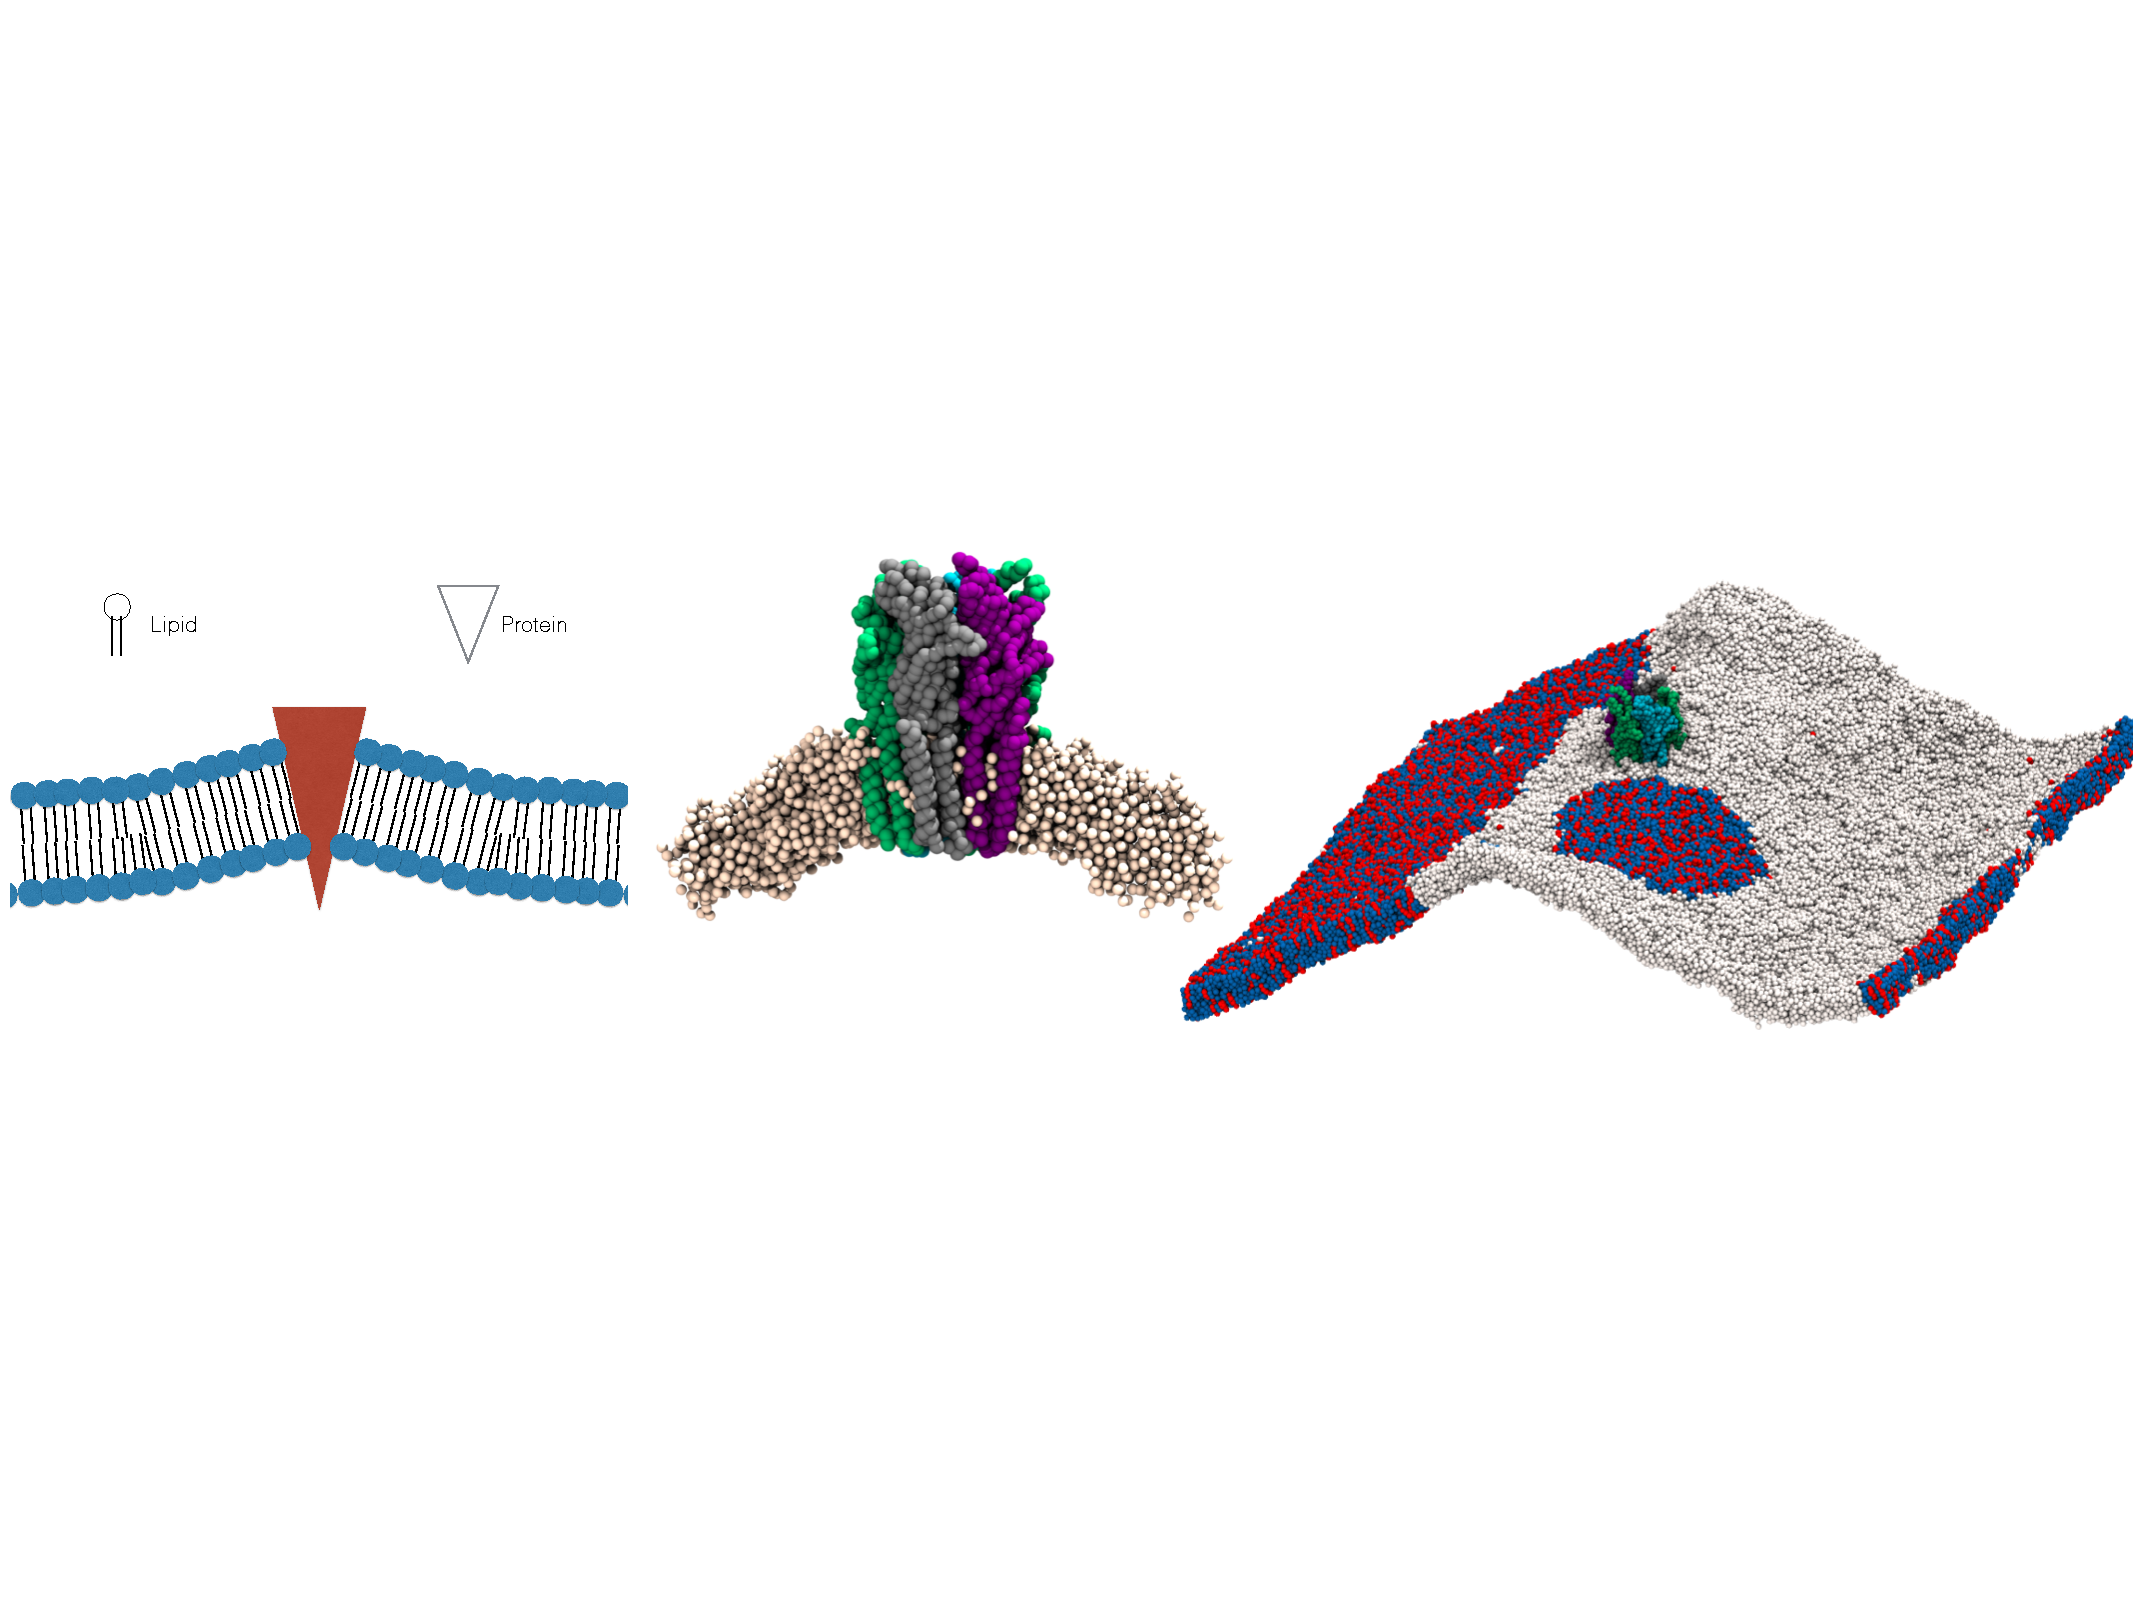
\includegraphics[width=1\linewidth]{./F31/Curvature4.pdf}
	\caption{Possible role of membrane flexibility in determining nAChR partitioning. (A) A schematic representation of predicted membrane deformation around a cone-shaped protein, as described in Goulian et al, \cite{Goulian1996} in which the protein imposes constraints on the slope of the membrane at the interface with the protein (B) Cross-sectional cut of simulation-frame showing membrane deformation around nAChR embedded in an $l_{do}$ phase composed of DHA-PE (white). (C) Phase-boundary partitioning in a larger membrane. nAChR is localized at the interface between the $l_{do}$ phase composed of DHA-PE and the $l_o$ phase composed of DPPC (blue) and cholesterol (red). Provided the membrane is sufficiently large, partitioning at the boundary permits tangential interaction with the cholesterol-rich $l_o$ domain while the flexible $l_{do}$ domain still absorbs the energetic cost of deformation.}
	\label{fig:deform}
\end{figure}

\begin{figure}[t!]
	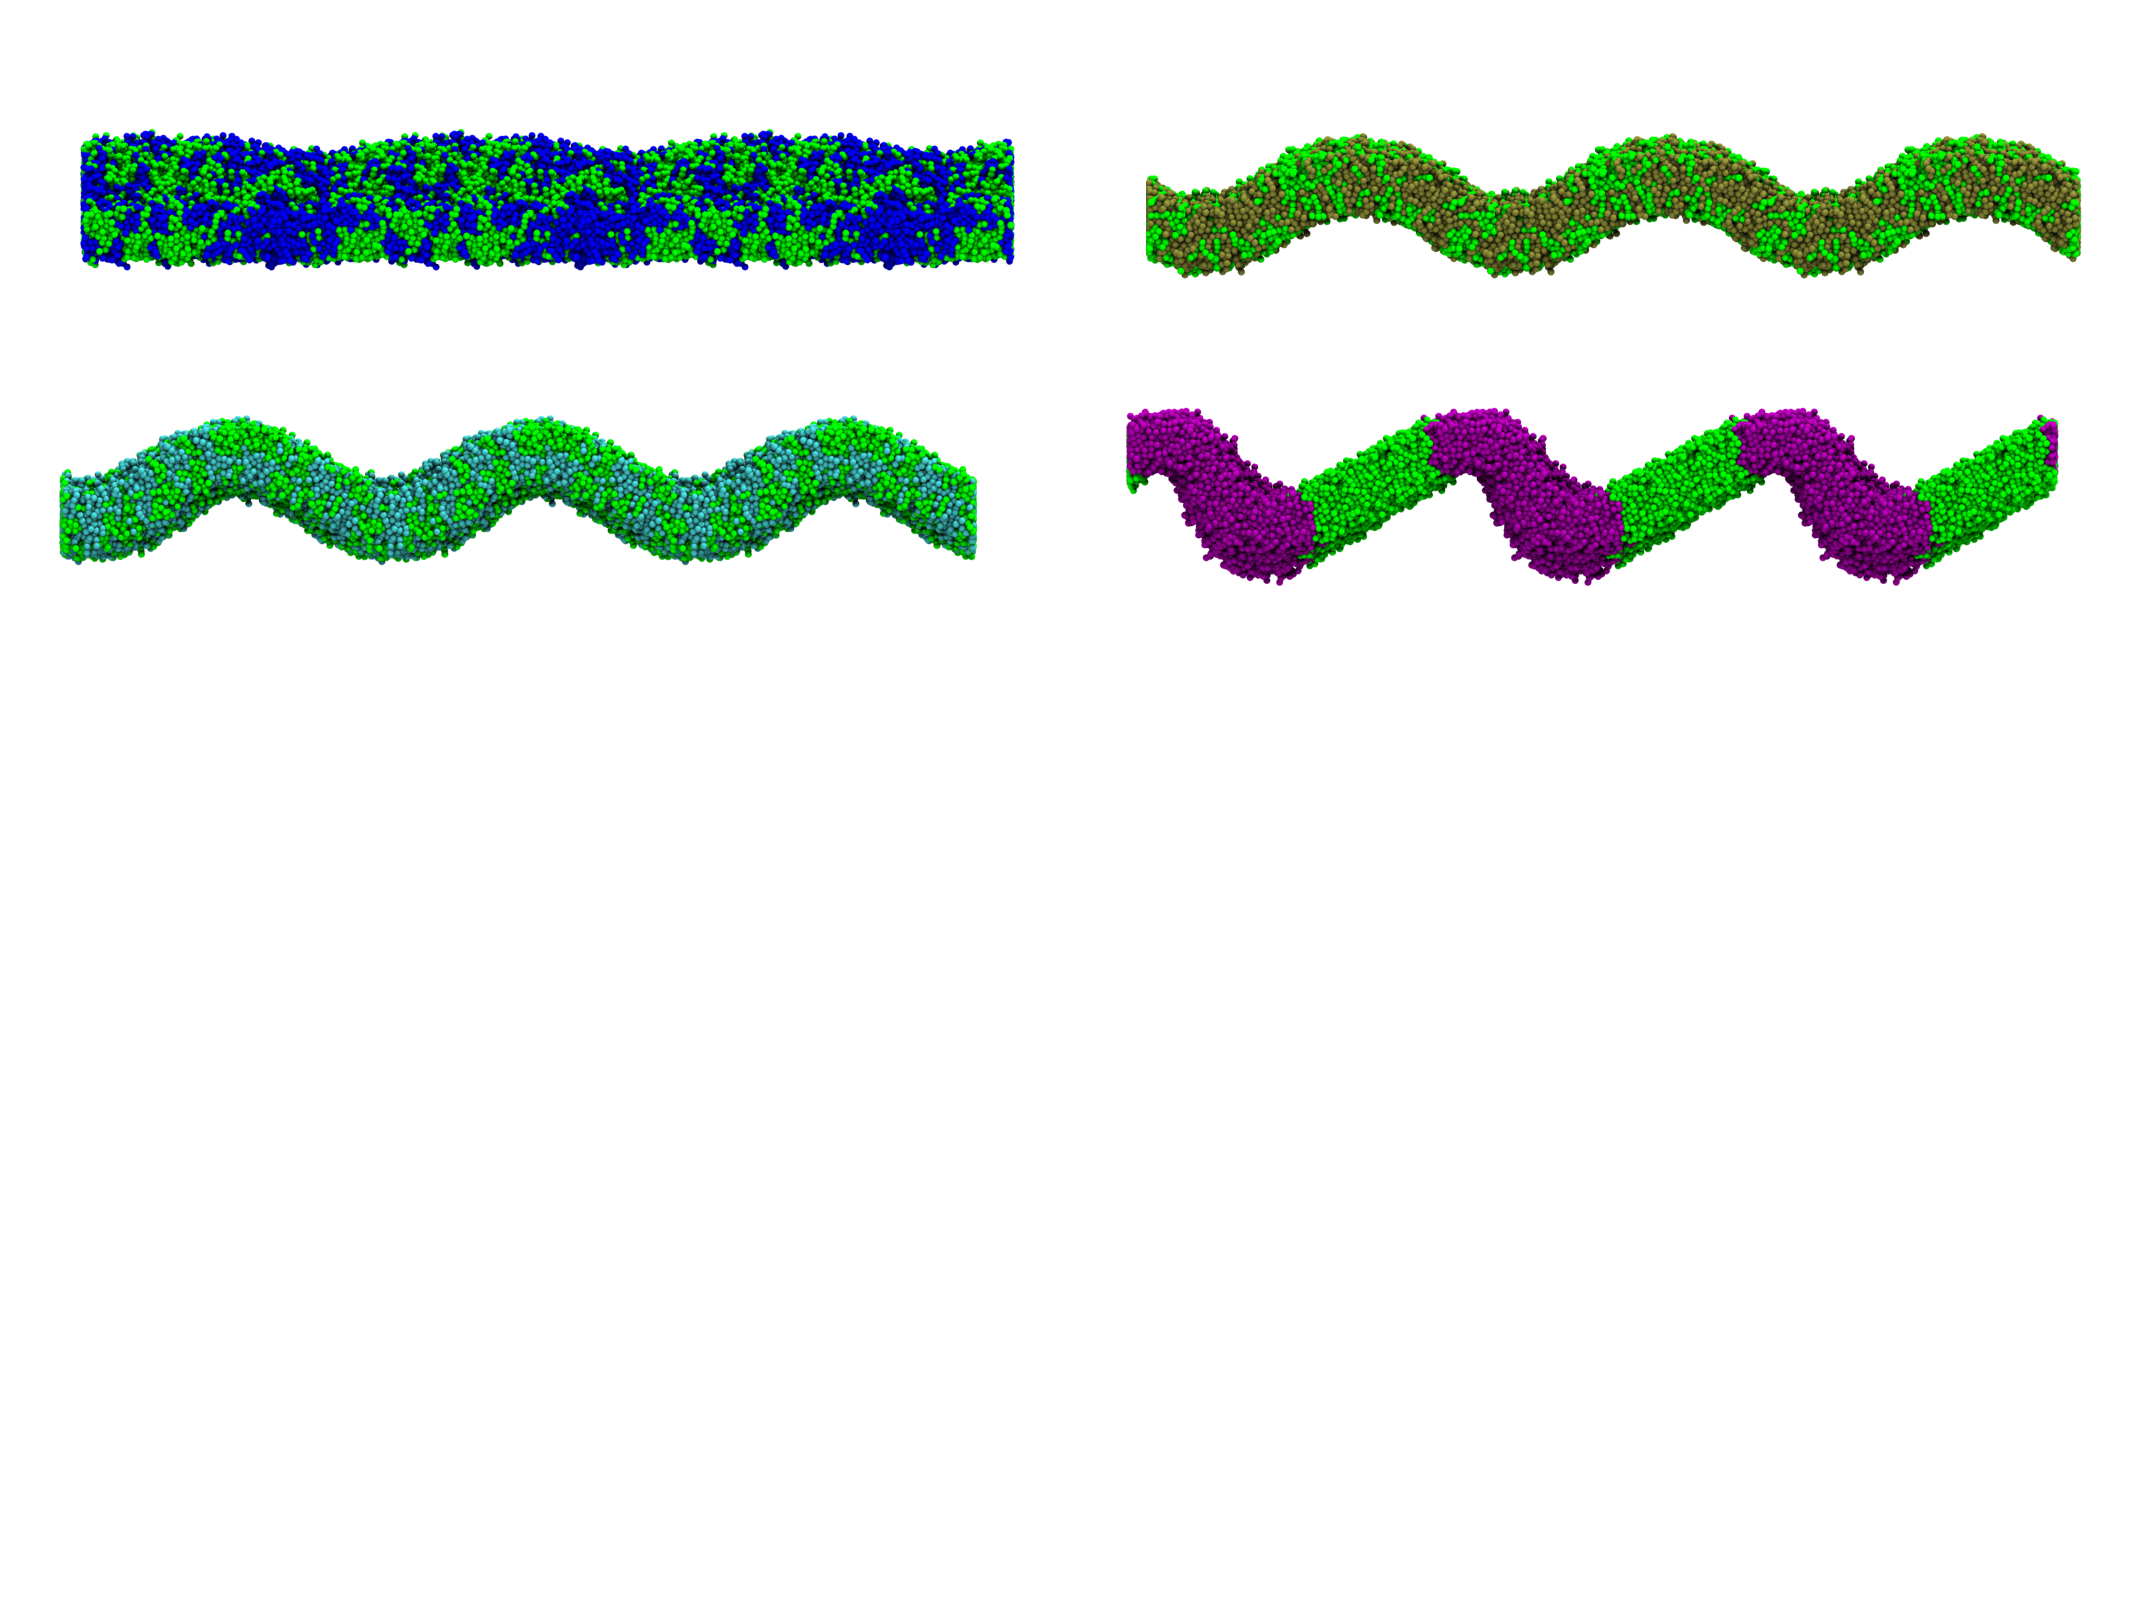
\includegraphics[width=1\linewidth]{./F31/MultiImageElastic.pdf}
	\caption{ Binary, randomly-mixed membranes with increasing thermal undulations and decreasing bending modulus $k_c$. We predict that the more flexible membranes (lower $k_c$) will accommodate a cone shaped protein with reduced energetic costs. The bending modulus $k_c$ can be measured from the thermal undulation spectrum, as well as additional methods appropriate for small membranes. Aim 3 proposes implementation of these methods into a plugin for the widely used analysis-software VMD. For the purpose of this image, saturated lipids are green, while unsaturated lipids are brown, cyan, and purple.}
	\label{fig:elast}
\end{figure}

As one example, neurotransmitter receptors must cluster at high density for efficient neurotransmission, and effects of lipid composition on membrane organization may serve an important modulatory role for an organism's ion channel functionality. The high density of nAChR clusters found in the postsynaptic membrane of the mature neuromuscular junction ($10^4$$\mu m^{-2}$) is well-established to be stabilized by dimerization of nAChRs via binding of the cytoplasmic peripheral membrane protein rapsyn \cite{Zuber_Structure_2013}. This process is also sensitive to membrane composition, particularly cholesterol. It has been frequently hypothesized \cite{Zhu2006,Bruses2001} that initial stages of clustering may require clustering via lipid domains, but experiments investigating whether nAChRs partition into lipid domains have been inconclusive \cite{Bermdez_Partition_2010,Perillo2016}.

Such experiments have focused primarily on detecting partitioning into liquid-ordered ($l_o$ ) domains, which is often detected differently than partitioning into $l_{do}$ domains; in my preliminary simulations we observe partitioning of nAChRs into the $l_{do}$ domain (Figure \ref{fig:ooct}). Partitioning into $l_{do}$ domains would also cluster receptors and be cholesterol dependent, but would be a less effective mechanism in low cholesterol membranes, such as oocytes.

%\subsection{Innovation of Research}

Our observation that nAChR partitions into $l_{do}$ domains was surprising because these domains are very low in cholesterol; the simplest hypothesis to explain cholesterol-sensitivity of nAChR function and oligomerization was that nAChR would partition to the cholesterol rich $l_o$ “raft” phase, although experimental data has been inconclusive.

Direct visualization, using computational microscopy, of the $l_{do}$ domain around nAChR in the MD simulation trajectories revealed a deformation of the membrane around the cone-shape of the TMD (Figure \ref{fig:deform}). This type of deformation was predicted for a general cone shape protein two decades earlier, based on analytical elasticity theories of protein-induced membrane deformations \cite{Goulian1996,Weikl1998} but has not, to our knowledge, been used to predict partitioning preferences of proteins. According to these theories, the energetic penalty for the membrane deformation should increase with the bending rigidity $k_c$, so a significantly more flexible $l_{do}$ phase would be the natural preferred phase for a single receptor.

My approach for this aim is to better determine the role of membrane flexibility in pLGICs partitioning; this has not previously been considered in simulation or experimental design, but it will provide essential insight into whether domain preferences are likely to be more sensitive to pLGIC sequence or to differences in domain rigidity.

%\subsection{Approach of Research}

If partitioning of pLGICs within domain-forming membranes is driven by membrane elasticity and the requirement for a flexible membrane around the cone-shaped protein, partitioning will be strongly sensitive to changes in lipid composition that affect flexibility or spontaneous curvature of $l_o$ and/or $l_{do}$ phases, and only weakly sensitive to pLGIC sequence, since pLGICs are structurally conserved. For example neuromuscular nAChR and GABA(A) receptor$ \alpha 1\beta 3\gamma 2$ $\alpha$ subunit's TMD share $\sim 20 \%$ identity \cite{jalv}, however it is unclear why either partition similarly. If partitioning is instead driven by specific interactions with lipids, it will be far more sensitive to pLGIC sequence, particularly the presence of bulky versus small residues in the TMD. 

My approach will involve first choosing purposeful pLGIC (GABA(A) receptor, glycine receptor, 5HT-3 receptor, and prokaryotic pLGICs such as GLIC or ELIC). Next, using multiple  multiple mutations to nAChR M1, M3, and M4 helices, to sequences of these other pLGICs. Lastly, adjust relative membrane elasticity parameters by e.g. increasing or decreasing membrane asymmetry or increasing or decreasing chain length. The effects of modifications on differences in elastic parameters will be quantified using the approach developed in Aim 3.

%As an example, comparing the sequence of TMDs for $\alpha$ subunits of neuromuscular nAChR and GABA(A) receptor$ \alpha 1\beta 3\gamma 2 $ shows $\sim 20 \% $ identity \cite{jalv}. Potentially suggesting that GABA(A) may not partition into the $l_{do}$. Interestingly the initial ternary DPPC:PUFA:CHOL membranes simulations show GABAAR with similar partitioning as nAChR. GABA(A) is currently running in an oocyte composition as a comparison. 
\subsection{Aim 3: Development and release of a user-friendly VMD plugin for measuring elastic parameters of heterogenous membranes}
While multiple individuals have developed scripts to determine the fluctuation spectrum of membranes, there is no universal tool computational chemists and biophysicists can use. I will develop a tool to measure elastic parameters and fluctuation spectra within the convenient scripting environment of the VMD software, which will alleviate the daunting nature of solving for the fluctuation spectrum and related moduli.  This tool will assist us in optimizing lipid selections for modeled neuronal membranes; I can adjust lipid species and lipid concentrations to mimic elastic properties of neuronal membranes.

This package could be of significant use to both biochemists and biophysicists. It would allow them to easily predict the elasticity properties of a membrane composed of non-specific lipids. Combined with VMD’s convenient scripting environment, this alleviates the daunting nature of solving for the fluctuation spectrum and related moduli, and promotes consideration of elastic effects in mechanisms by relying on the Monge Gauge $h(r)=z$, where z is a deviation in membrane height from 0.  

%\subsection{Innovation of Research}

Numerous computational methods with increasing sophistication for measuring elastic properties of membranes have been developed by physicists and physical chemists \cite{Galimzyanov_Undulations_2017,Brannigan2006,Pan_Effect_2009,Rawicz_Effect_2000,Goetz1999}. However, most are developed using in-house code, and none are integrated into a widely-used, flexible analysis package such as VMD \cite{HUMP96}.

I will develop a user-friendly VMD plugin that can measure elastic properties for generalized heterogeneous lipid bilayers, allowing comparison among different lipid compositions relying on measurement techniques in the convenient scriptable VMD environment. It will allow those with a need to quantify membrane flexibility, but without the requisite skills in lower-level programming or background in soft-condensed matter physics, to carry out reliable and straightforward calculations. It will also link the elasticity calculations to the extensive abilities of VMD for analyzing molecular interactions.

%\subsection{Approach of Research}

I envision the proposed plugin will be usable from both a GUI and VMD’s tk terminal, and will provide the option to measure the bending modulus, stretching modulus, tilt modulus, equilibrium area per molecule, and monolayer spontaneous curvature, based on fluctuation spectrum methods \cite{Brannigan2006,Goetz1999} and molecular fluctuations \cite{Galimzyanov_Undulations_2017,Rawicz_Effect_2000,Pan_Effect_2009}. Calculations will be performed on a trajectory loaded through VMDs extensive trajectory format libraries, making analysis convenient for users of NAMD, GROMACS, LAMMPS, HOOMD, or any MD software that outputs in one of the many VMD-readable formats.

The analysis code will have the option to specify starting and ending frames, as well as how to approximate the membrane surface and/or lipid tilt angles simply based on VMD-based atom selections, greatly simplifying the required code. The plugin will serve as a wrapper to C code that performs fast Fourier transforms and spectral analysis. Data will be output to a an ASCII file that can be easily manipulated in a scientific programing language of the user’s choice (i.e. Python, Matlab).

Data will be collected by binning over a membrane with adjustable bin steps ($dx$ and $dy$), and averaging the membrane hight ($z$) over the bin. Setting $z$ to $h(r)$ (where $r=r(x,y)$) and performing a Fourier transform on $h(r)$ results in $\tilde{h}(q)$,
	\begin{equation}
		\begin{aligned}
		\tilde{h}(q)=\frac{1}{L}\int dr (h(r) e^{-i q r})\\
		h(r)=\frac{1}{L}\sum \tilde{h}(q) e^{i q r}
		\label{eq:For}
		\end{aligned}
	\end{equation}
where $q$ is the spacial frequency. Allowing F to be the Helfrich Hamiltonian
\begin{equation}
  \begin{aligned}
    F = k_c(H-2C_0)^2+k_GK,
  \end{aligned}
\end{equation}
where, $k_c$ is the bending modulus, $H$ is the mean curvature, $k_G$ is the Guasian modulus, and $K$ is the Gausian curvature. When applied to a closed membrane $C_0,k_G,K$ drop out, and the equation reduces to 
\begin{equation}
  \begin{aligned}
    F = k_cH^2,
  \end{aligned}
\end{equation}
where H can be expressed as
\begin{equation}
  \begin{aligned}
    H = |\nabla^2h(r)|.
  \end{aligned}
\end{equation}
We can then determine the fluctuation spectrum, $S(q)$, which \cite{Goetz1999} defined as
  \begin{equation}
    \begin{aligned}
      S(q)=\langle|\tilde{h}(q)|^{2}\rangle.
    \end{aligned}
    \label{eq:s1}
  \end{equation}
According to Helfrich elasticity of membranes,\cite{safran2003statistical} at long wavelengths the spectrum should obey approximate to 
  \begin{equation}
    \begin{aligned}
      S(q)\sim\frac{k_BT}{k_c q^4}%%+\frac{k_BT}{\sigma q^2}.
    \end{aligned}
    \label{eq:s2}
  \end{equation}
Where $k_B$ is Boltzmann's constant, $T$ is temperature, and $k_c$ is the bending modulus.

We would work with VMD developers to incorporate the plugin into the official VMD distribution, and provide support to the VMD user’s community, as well as necessary updates and improvements.

\printbibliography
\end{document}
